\newline
\newline
\vspace{3mm}
\hfill

\section{Introduction}

\hspace{2cm}In this chapter we discuss software architecture in the project, services, back-end and front-end architecture.
Web services are used in communication between users (customers and vendors) of the website and mobile application and the robot.
By sending a request to the server containing specific data then waiting for the appropriate response to send it to the robot server to perform the wanted action which will be a position the robot will go to.
We will describe the functionality of each part of the software system, including database to store the users, order, vendor’s products and robot location.


\section{Software Architecture}
\hspace{2cm}This Diagram Describe Software Architecture of our web site \ref{fig: LMD}
\begin{figure}%
    \center%
    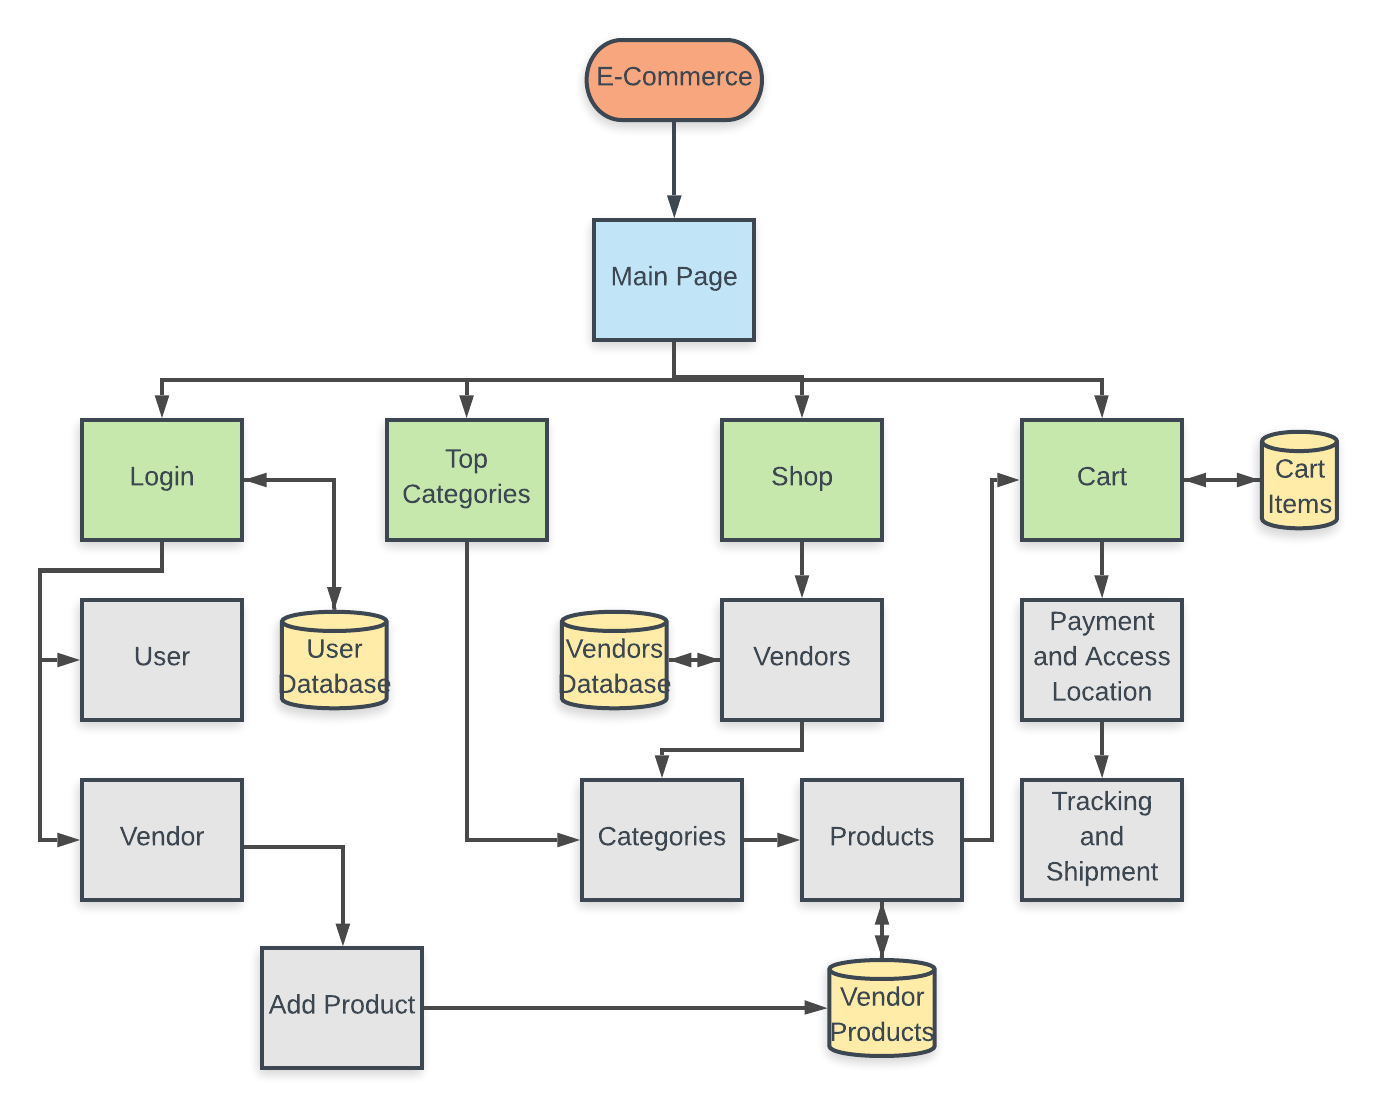
\includegraphics[width=1\textwidth]{images/Software/frontend.png}%
     % you need to add the caption for the list of figures
    \caption[LMD Software Architecture]{LMD Software Architecture}\label{fig: LMD}%
  \end{figure}

 
\begin{figure}[htp]%
    \center%
    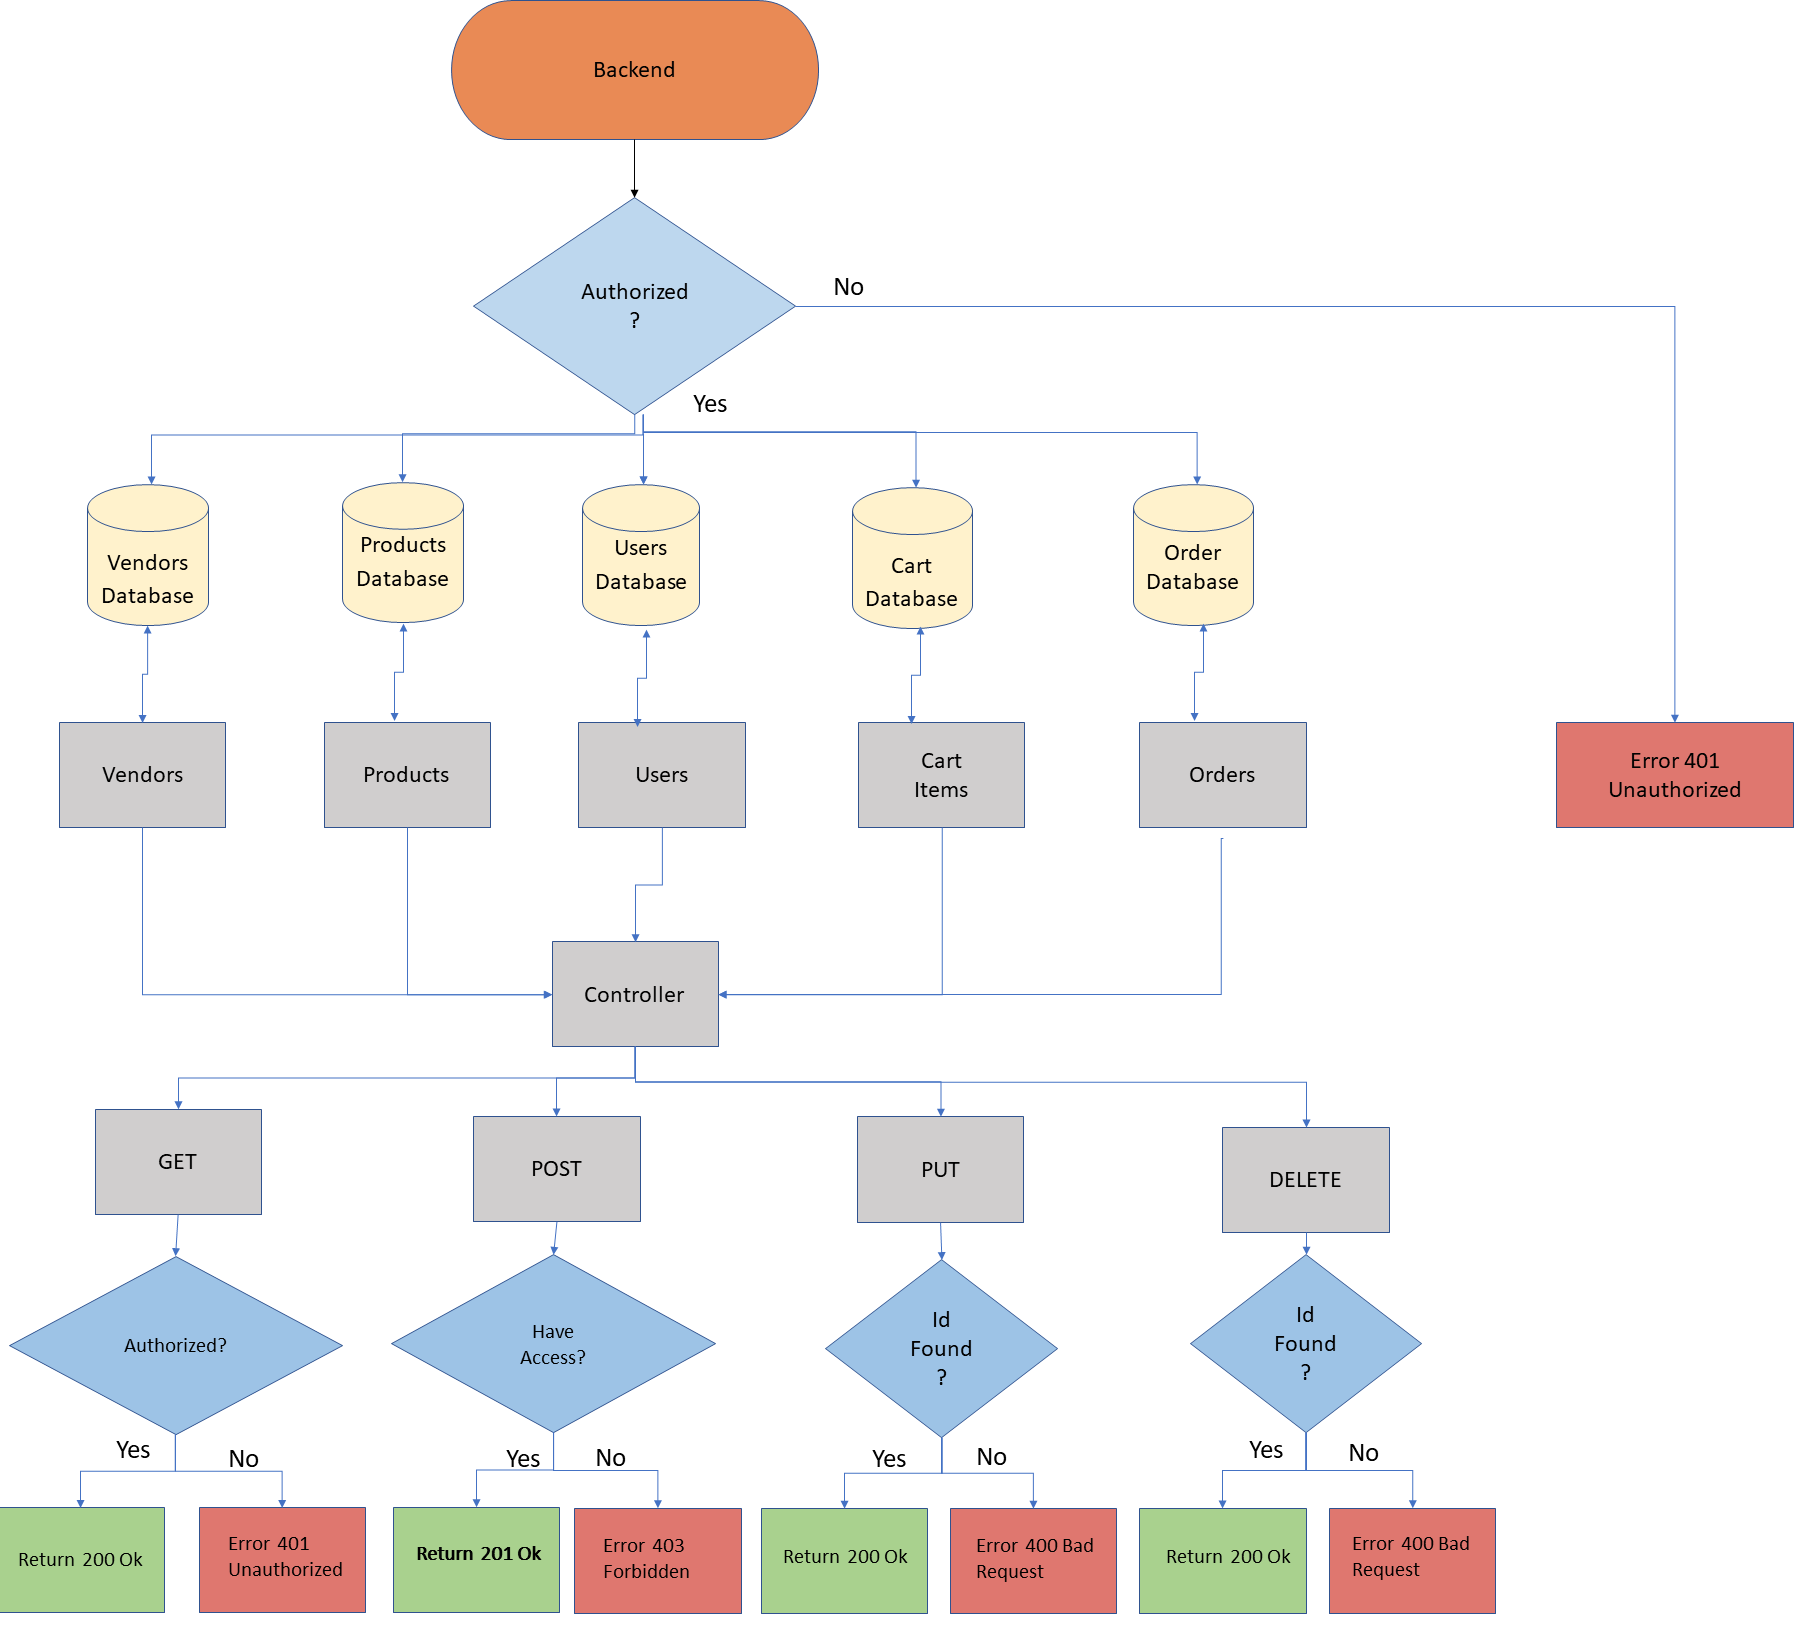
\includegraphics[width=1\textwidth]{images/Software/backend1.png}%
     % you need to add the caption for the list of figures
    \caption[Back End]{Back End}\label{fig: Back End}%
  \end{figure}




\section{Back-end Architecture}
\hspace{2cm}Back-end is all of the technology required to process the incoming request and generate and send the response to the client. This typically includes three major parts:
    \begin{enumerate}
    \setcounter{enumi}{0}
    \item Server that receives the request.
    \item Application. This is the application running on the server that listens for the requests, retrieve the data from the database and send the response to the user.
    \item Database that is used to store and organize the data
    \end{enumerate}
    
We use NodeJs write the server side application which is an open-source, cross-platform JavaScript run-time environment that executes JavaScript code outside of a browser to produce dynamic web page content before the page is sent to the user's web browser.
Express package is a minimal and flexible Node.js web application framework that provides a robust set of features for web and mobile applications. We use it  to  set up middlewares, to respond to HTTP Requests to Define a routing table which is used to perform different actions based on HTTP Method and URL 
and to dynamically render HTML Pages based on passing arguments to templates.

\subsection{Server}
\hspace{2cm}Is a computer designed to process requests and deliver data to another computer, called “Clients ” over the internet or a local network, This architecture called client-server model. In this model server serve the data from client.

The nature of communication between server and client  in “request-and-response”.
\begin{figure}%
    \center%
    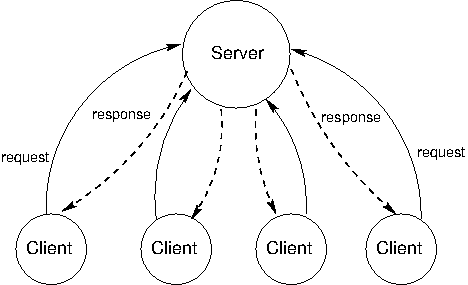
\includegraphics[width=1\textwidth]{images/Software/clientserver.png}%
     % you need to add the caption for the list of figures
    \caption[Client and Server Communication]{Client and Server Communication}\label{fig: login}%
  \end{figure}
  
 Server runs an app that contains logic about how to respond to various requests based on the HTTP verb and the Uniform Resource Identifier (URI). The pair of an HTTP verb and a URI is called a route and matching them based on a request is called routing.
The data that the server sends back can come in different forms. For example, a server might serve up an HTML file, send data as JSON, or it might send back only an HTTP status code. You’ve probably seen the status code “404 - Not Found” whenever you’ve tried navigating to a URI that doesn’t exist.

\subsection{Application Architecture}
\hspace{2cm}Web application development uses a 3-tiers MVC (model-view-controller) design pattern.it provide three main layers; model, view , controller. MVC pattern separates the characteristic of the application which makes it easy for us to test our application as relation among different components of the application. These tiers describe as shown in figure
\begin{figure}%
    \center%
    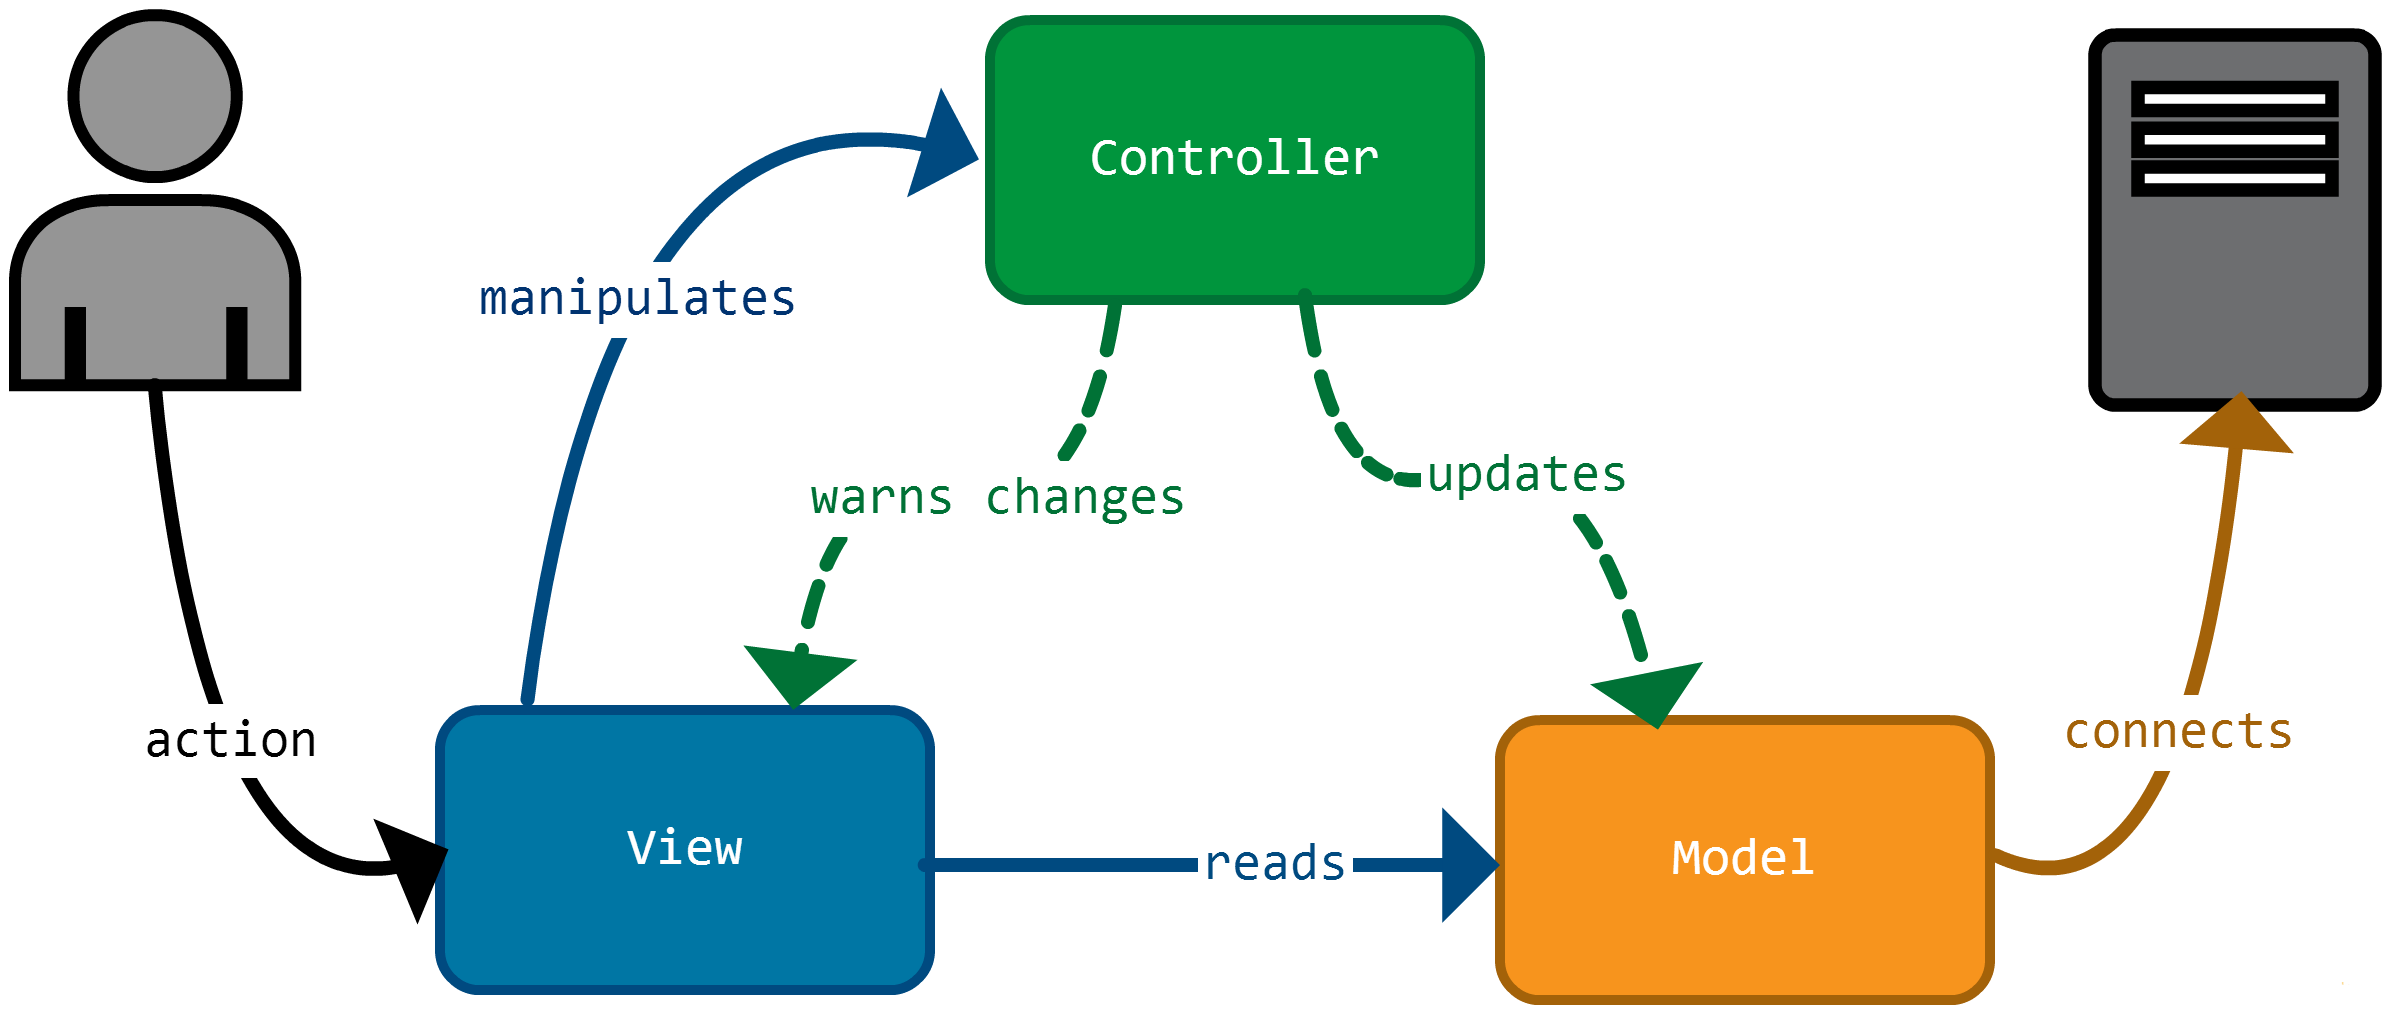
\includegraphics[width=1\textwidth]{images/Software/MVC2.png}%
     % you need to add the caption for the list of figures
    \caption[Web based application]{Web based application}\label{fig: login}%
  \end{figure}
\begin{enumerate}
    \setcounter{enumi}{0}
    \item Model :- Model component corresponds to all the data-related logic that the user works with. This can represent either the data that is being transferred between the View and Controller components or any other business logic-related data. It is used to retrieve, insert or update the data into the database associated with our application. An example of the code to connect to the database is given below :
\begin{figure}%
    \center%
    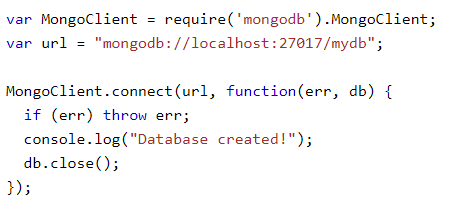
\includegraphics[width=1\textwidth]{images/Software/Capture.PNG}%
     % you need to add the caption for the list of figures
    \caption[Database Communication]{Database Communication}\label{fig: login}%
  \end{figure}
  
    \item View:- in a web-based application is representation of the user-interface (UI). Buttons, forms and other information visible to the user on the web are all part of View.  By using that interface users interact with our application. These Views are generally bind from the model data and have extensions such as html, aspx, cshtml,
    vbhtml, etc.
    
    \item Controllers:- act as an interface between Model and View components to process all the business logic and incoming requests, manipulate data using the Model component and interact with the Views to render the final output. So when the user clicks on the hyperlinks in the web page , the controlled receive the request and determine which model to call, and it confirms to use which view to display the returning data of the model processing.
    \end{enumerate}  

 
 Our website has many controllers:
  \begin{enumerate}
    \setcounter{enumi}{0}
    \item Customers Controller: uses many apis to get and update and delete and create new customer in our system. Apis are:
    \begin{itemize}
    \item GET /api/customers: To get all customer 

    \item POST /api/customers: To create new Customers

     \item DELETE /api/customers/:id: To delete Customers \newline
    \end{itemize} 

    \item Vendors Controller: uses many apis to get and update and delete and create new Vendor in our system. Apis are :
    \begin{itemize}
    \item GET /api/vendors: To get all Vendors 

    \item POST /api/vendors: To create new Vendors

     \item DELETE /api/vendors/:id: To delete Vendors
     
     \item PUT /api/vendors/:id: To update specific vendor \newline

    \end{itemize}
    
    \item Products Controller: uses many apis to get all products and update the data of a product of specific vendor,delete a product of specific vendor and create new products to the chosen vendor. 
	Apis are :
	\begin{itemize}
    \item GET /api/products: To get all products
    \item POST /api/products: To Create new product
     \item DELETE /api/products/:id: To delete product of specific vendor
     \item PUT /api/products/:id: To update product of specific vendor \newline
    \end{itemize} 

    \item Orders Controller: uses many apis to get all orders made by the users, update and delete the data of orders before it being shipped to customer, and create new orders that included many products of the vendors in our system.
    \begin{itemize}
    \item GET /api/orders: To get all Orders
    \item POST /api/orders: To Create new Orders
     \item DELETE /api/orders/:id: To delete specific Order
     \item PUT /api/orders/:id: To update specific Orders
     \newline
    \end{itemize} 
    
    \item Robot Controller: will be used in the future when we have more than one Robot. Each robot will have unique ID. So when we make an order, routing algorithm can be used to choose the free and the nearest robot to deliver the order.\newline
    
    \item Cart Controller: is used to get all items Which has been selected for purchase by specific user. it is used also to add new items or delete items from the cart of the authenticated user. \newline

    \item Payment Controller: will allow individuals and businesses to make and receive payments over the Internet. It will provide the technical, fraud prevention, and banking infrastructure required to operate online payment systems.\newline

    \item Users Controller: gets all users in our system included vendors and customers.\newline
    
    \item Authentication Controller: allows users to log in to the system. So when user enters the E-mail and the password, post request is used to check the Data in the body of the request to verify the user.
Once user is logged in, each request will include token, allowing the user to access routes, services, and resources that are permitted with that token. 
Authentication can be made by many methods, in our system authentication is made using JSON Web Token (JWT).\newline \hfill \break
\textbf{JSON Web Token} (\textbf{JWT}) \cite{JWT}:
is an open standard (RFC 7519) that defines a compact and self-contained way for securely transmitting information between parties as a JSON object. This information can be verified and trusted because it is digitally signed. JWTs can be signed using a secret (with the \textbf{HMAC} algorithm) or a public/private key pair using \textbf{RSA} or \textbf{ECDSA}.\newline
JSON Web Tokens looks like the following: xxxxx.yyyyy.zzzzz and consists of three parts separated by dots (.) which are:
\begin{enumerate}
    \setcounter{enumi}{0}
    \item Header: typically consists of two parts: the type of the token, which is JWT, and the signing algorithm being used, such as HMAC SHA256 or RSA
    \item Payload: contains the claims. Claims are statements about an entity (typically, the user) and additional data. There are three types of claims: registered, public, and private claims.
    \item Signature: To create the signature part you have to take the encoded header, the encoded payload, a secret, the algorithm specified in the header, and sign that. The signature is used to verify the message wasn't changed along the way, and, in the case of tokens signed with a private key, it can also verify that the sender of the JWT is who it says it is.
    The figure \ref{fig: jwt} shows a JWT that has the header and payload encoded, and it is signed with a secret.
    \begin{figure}[htp]%
    \center%
    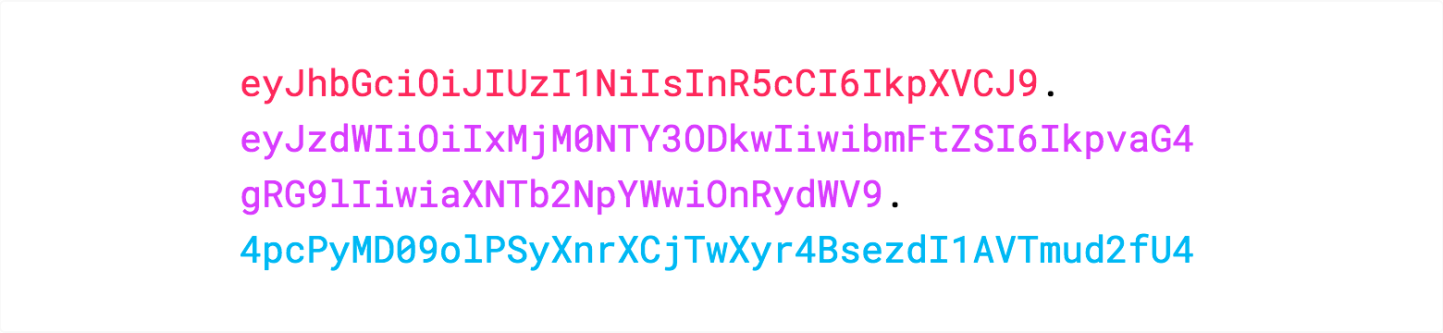
\includegraphics[width=1\textwidth]{images/Software/encoded-jwt3.png}%
     % you need to add the caption for the list of figures
    \caption[Encoded JWT]{Encoded JWT}\label{fig: jwt}%
  \end{figure}
    \end{enumerate}
    In figure \ref{fig: djwt} you can use decode JWT to  know the additional data about the user, and to define the type of the token.
 \begin{figure}[htp]%
    \center%
    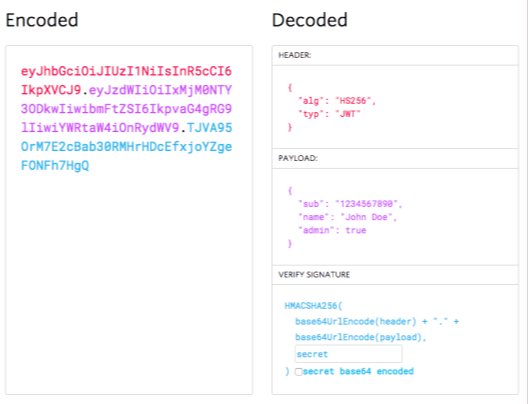
\includegraphics[width=1\textwidth]{images/Software/legacy-app-auth-5.png}%
     % you need to add the caption for the list of figures
    \caption[Encoded and Decoded JWT]{Encoded and Decoded JWT}\label{fig: djwt}%
  \end{figure}
    \end{enumerate} \newpage
    
\subsection{Database Architecture}
\hspace{2cm}This section illustrates the architecture of the database using NoSQL database. The figure \ref{fig: db schema} describes the tables created in the database. Each table has a primary key and a foreign key to connect to another table.
We used MongoDB is a cross-platform document-oriented database program. Classified as a NoSQL database program, MongoDB uses JSON-like documents with schema. Also Fields in a MongoDB document can be indexed with primary and secondary indices.
To validate the entered data we used Joi. Joi allows you to create blueprints or schemas for JavaScript objects (an object that stores information) to ensure validation of key information.
We define the input must be a string, number.. etc, if the input is required or not, if there is a specified regular expression such as emails and passwords.
\begin{figure}[htp]%
    \center%
    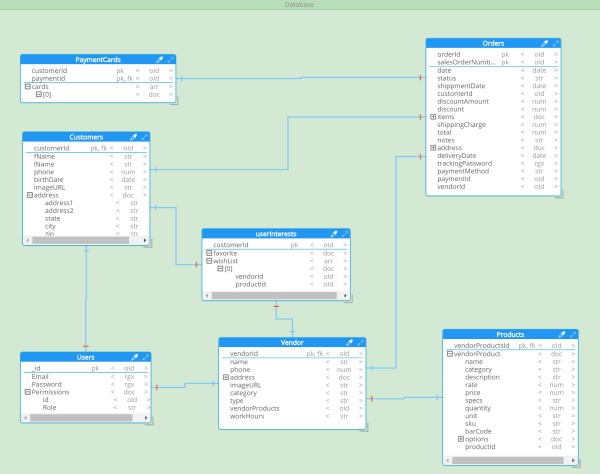
\includegraphics[width=1\textwidth]{images/Software/dbSchema.jpeg}%
     % you need to add the caption for the list of figures
    \caption[DataBase Shcema]{DataBase Shcema}\label{fig: db schema}%
  \end{figure} \newpage
  

\section{Web Application Front-end}
\hspace{2cm}Front-end web development, also known as client-side development is the practice of producing HTML, CSS and JavaScript for Web Application so that a user can see and interact with them directly. 

We use React.Js which is a JavaScript library for building user interfaces as the basic architecture of React applies beyond rendering HTML element in the browser.
React applications usually require the use of additional libraries for state management, routing, and interaction with an API such as: semantic-ui which is framework designed for theming and axios HTTP requests from both browser and server. Axios is an npm library (originally short for Node Package Manager) is a package manager for the JavaScript programming language.

One of the advantages to use React is the use of a "virtual Document Object Model", or "virtual DOM". React creates an in-memory data-structure cache, computes the resulting differences, and then updates the browser's displayed DOM efficiently. This allows the programmer to write code as if the entire page is rendered on each change, while the React libraries only render subcomponents that actually change.

Now, we will add routes to the app. This time the Router will be rendered. We will also set components for each route.

As shown in figure \ref{fig: routes} we have these routes in the website.
\begin{figure}[htp]%
    \center%
    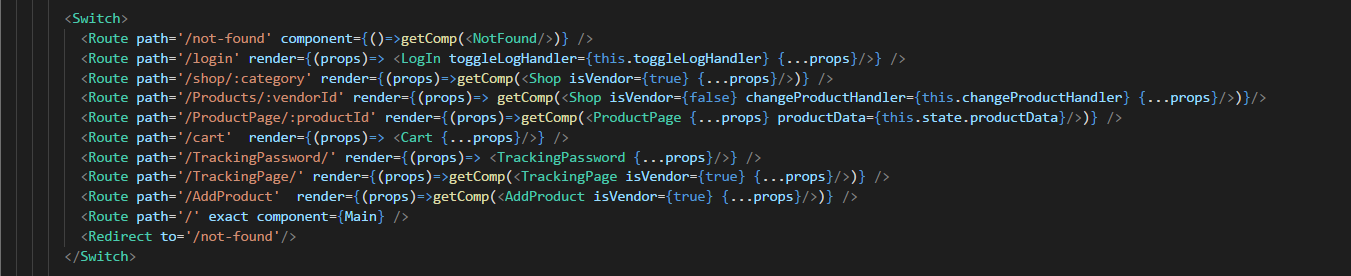
\includegraphics[width=1\textwidth]{images/Software/routes.PNG}%
     % you need to add the caption for the list of figures
    \caption[Website Routes]{Website Routes}\label{fig: routes}%
  \end{figure}

\textbf{Website Pages} 
In Figure \ref{fig: login} a login page to enter the email and password also checks that the user must be authorized.
\begin{figure}[htp]%
    \center%
    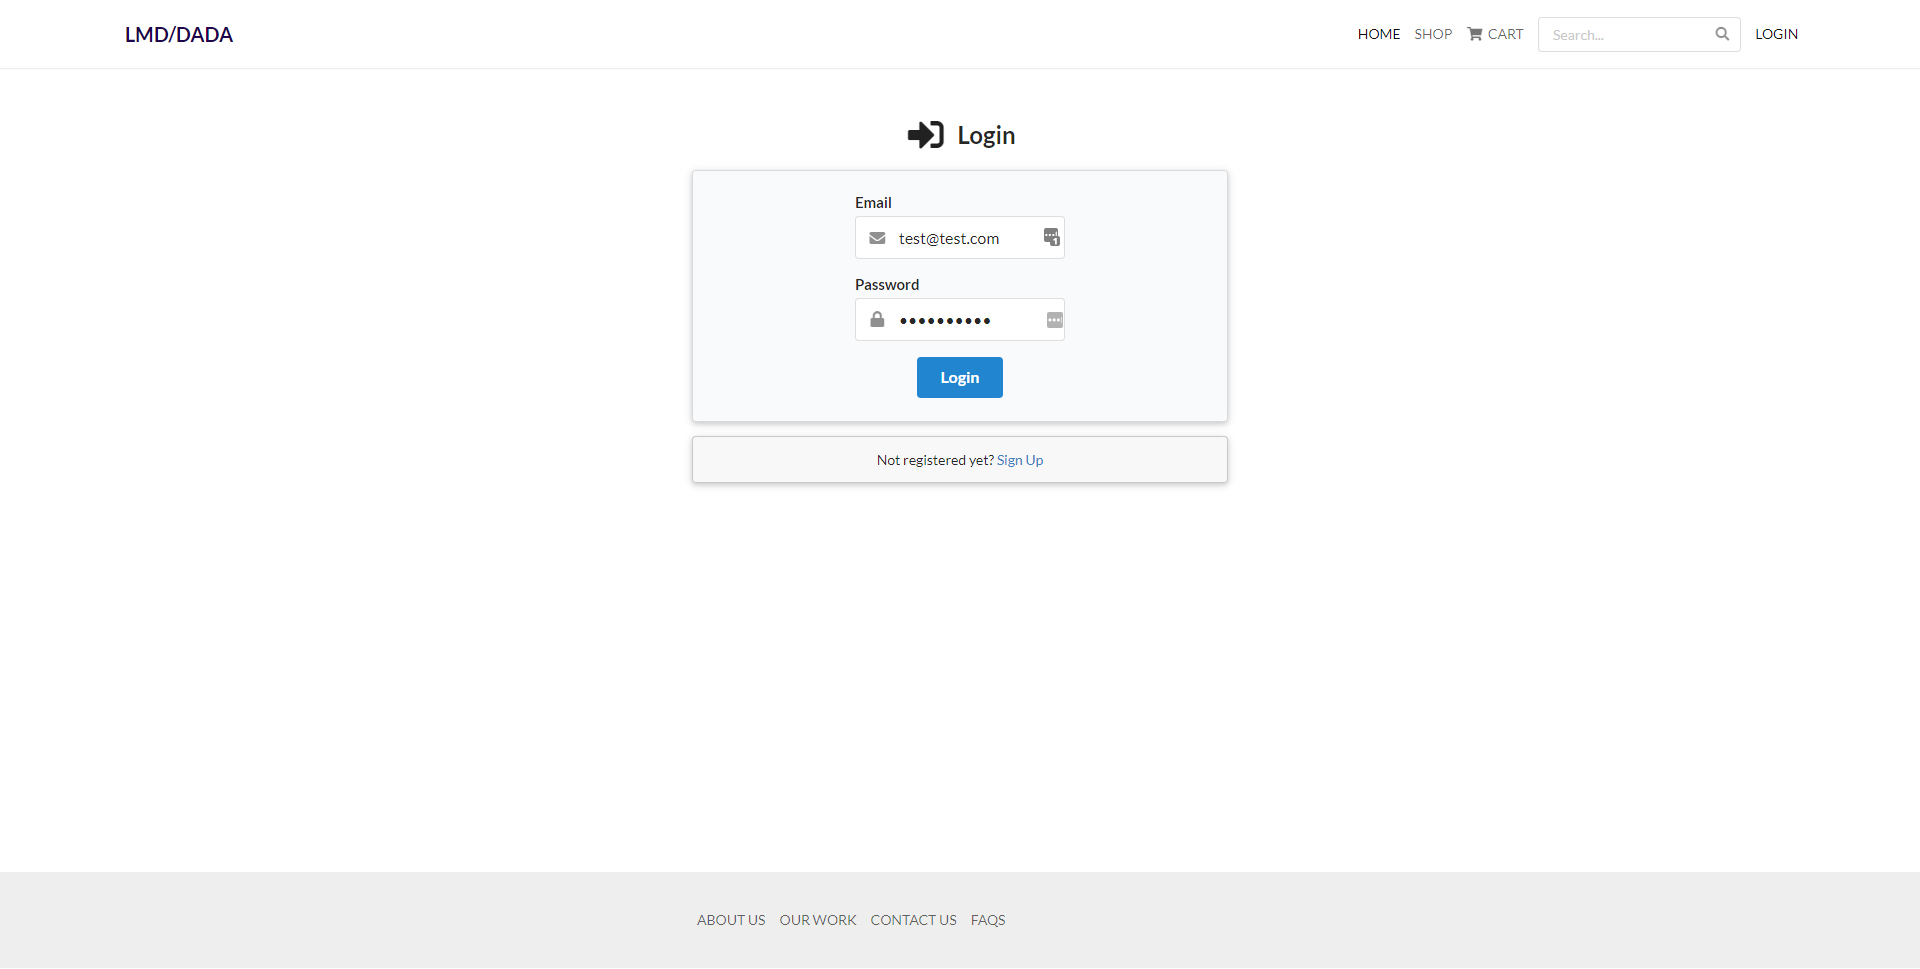
\includegraphics[width=1\textwidth]{images/Software/login.PNG}%
     % you need to add the caption for the list of figures
    \caption[Website: Login page]{Website: Login page}\label{fig: login}%
  \end{figure}

In Figure \ref{fig: main Page} main page contains our logo and top categories such as (Food, Health and Clothes), the user can access the shop, his cart or choose his favourite category.\newline \newline
\begin{figure}[htp]%
    \center%
    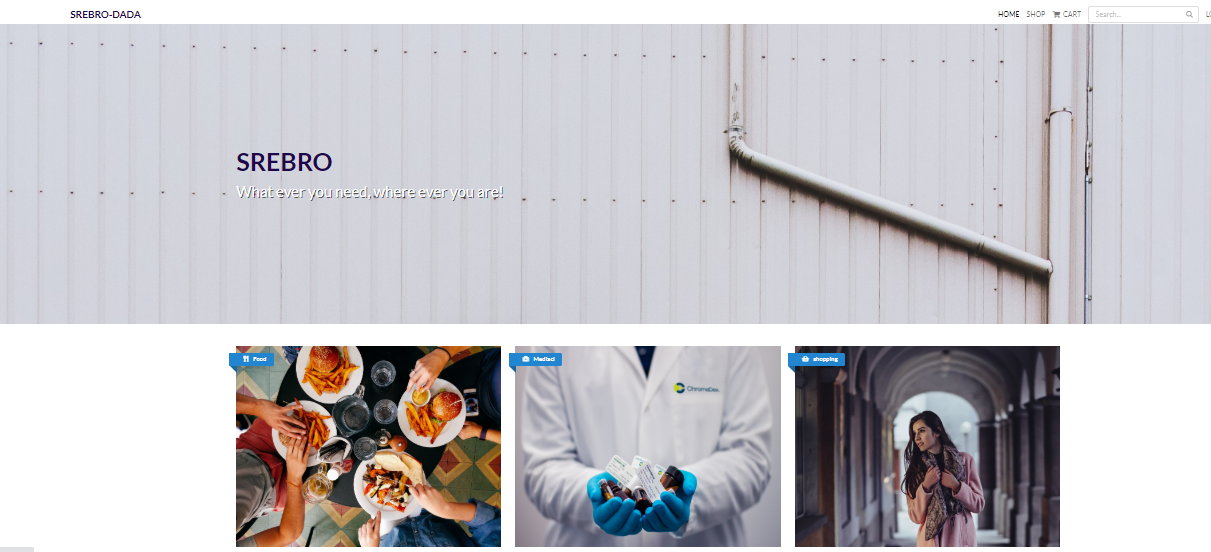
\includegraphics[width=1\textwidth]{images/Software/MainPage.PNG}%
     % you need to add the caption for the list of figures
    \caption[Website: Main Page]{Website: Main Page}\label{fig: main Page}%
  \end{figure}\newline \newline
 
In Figure \ref{fig: profile} profile page for the customer to be able to track his orders and recent activities. Also if the user is a vendor, "Add Product" button will be shown to enable him to add his products to be shown in the shop.
\begin{figure}[htp]%
    \center%
    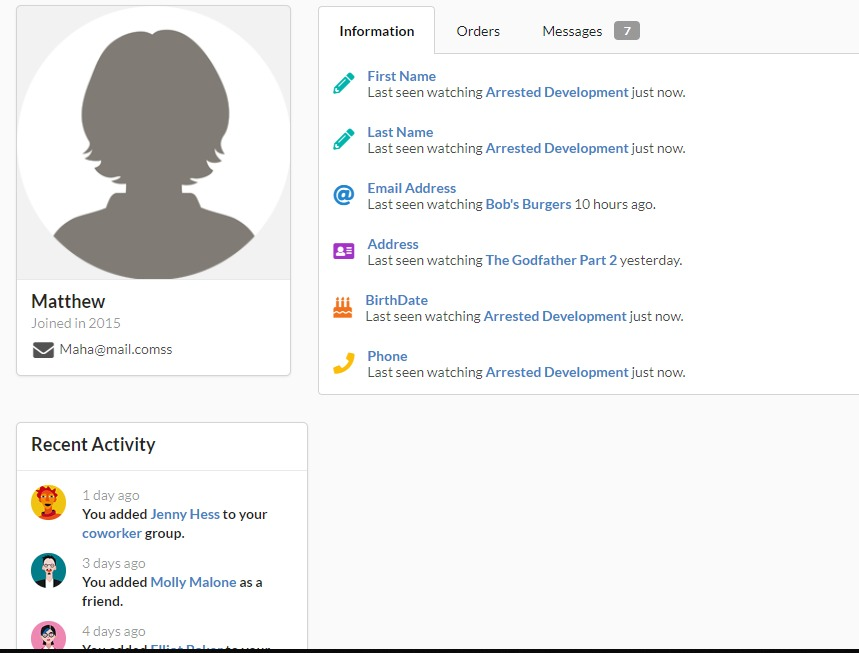
\includegraphics[width=1\textwidth]{images/Software/profile.jpeg}%
     % you need to add the caption for the list of figures
    \caption[Website: Profile Page]{Website: Profile Page}\label{fig: profile}%
  \end{figure}\newpage
  
In Figure \ref{fig: vendors}, \ref{fig: products} and \ref{fig: product Page} shop page has our vendors each contains their products with description provided it product page, search and filter by category are available while browsing and from product page the user can add this product to his cart.

  \begin{figure}[htp]%
    \center%
    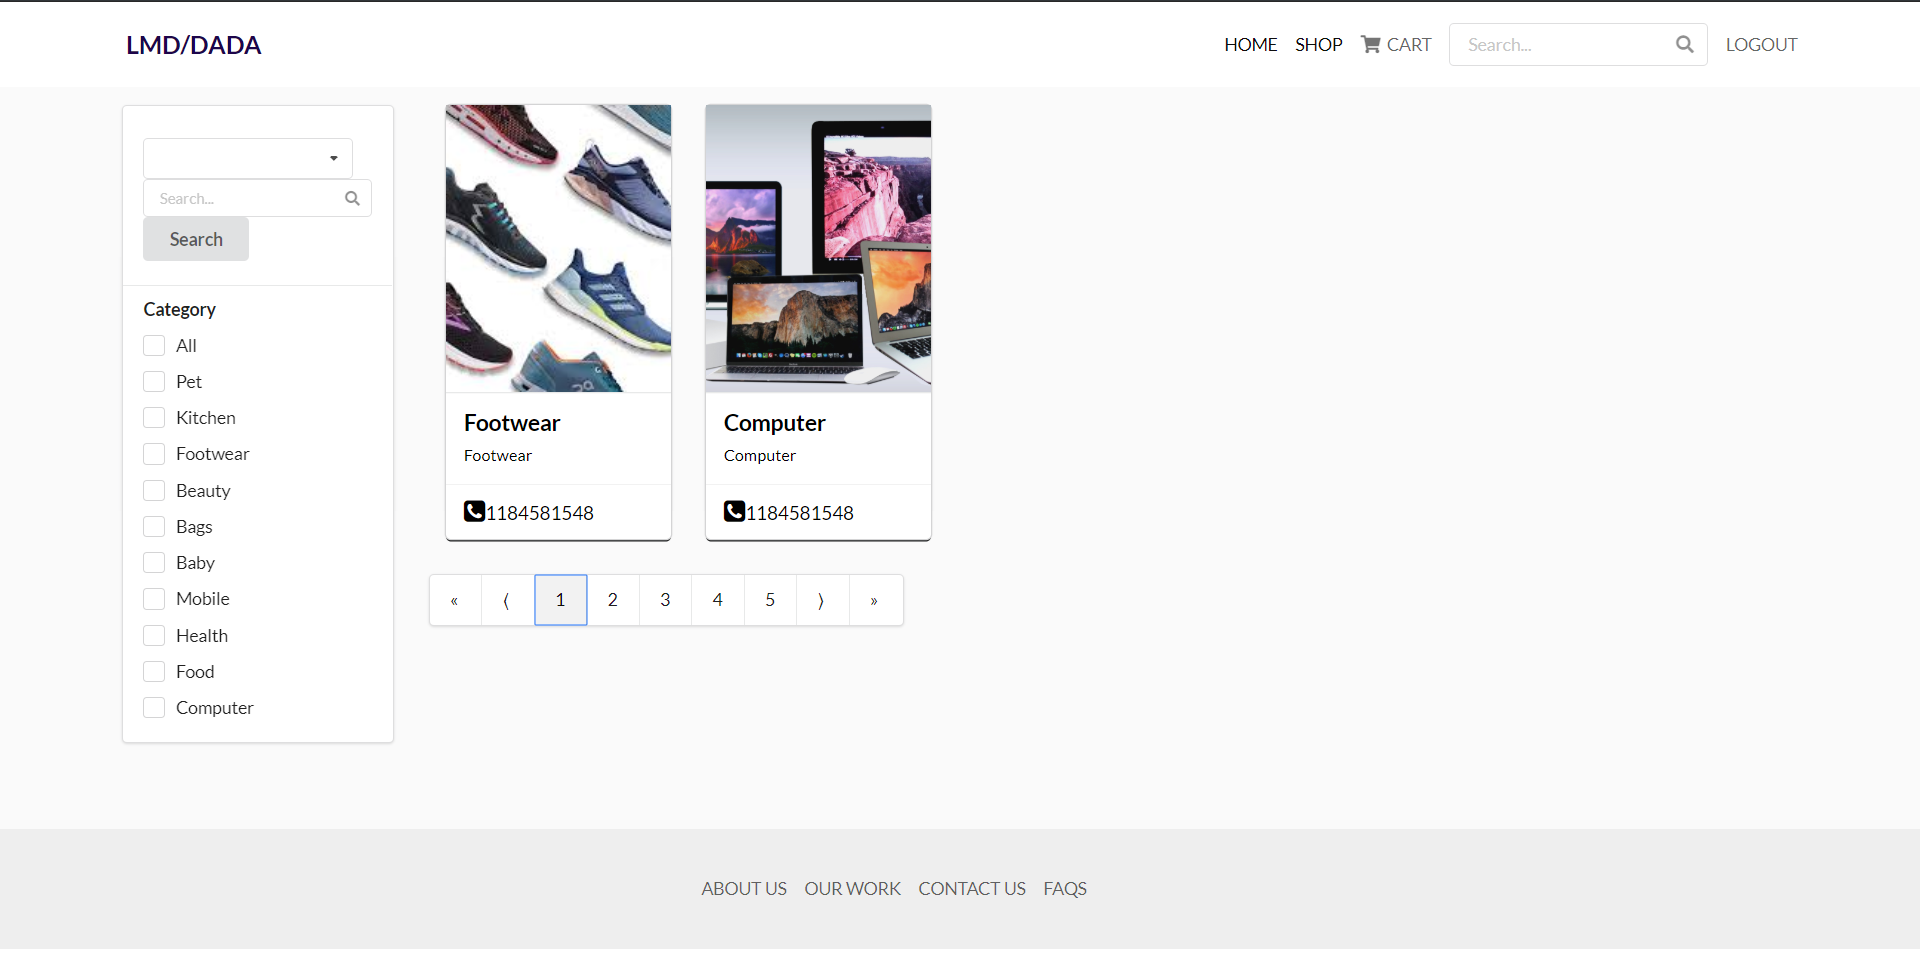
\includegraphics[width=1\textwidth]{images/Software/vendors.PNG}%
     % you need to add the caption for the list of figures
    \caption[Website: Vendors Page]{Website: Vendors Page}\label{fig: vendors}%
  \end{figure}
  
  \begin{figure}[htp]%
    \center%
    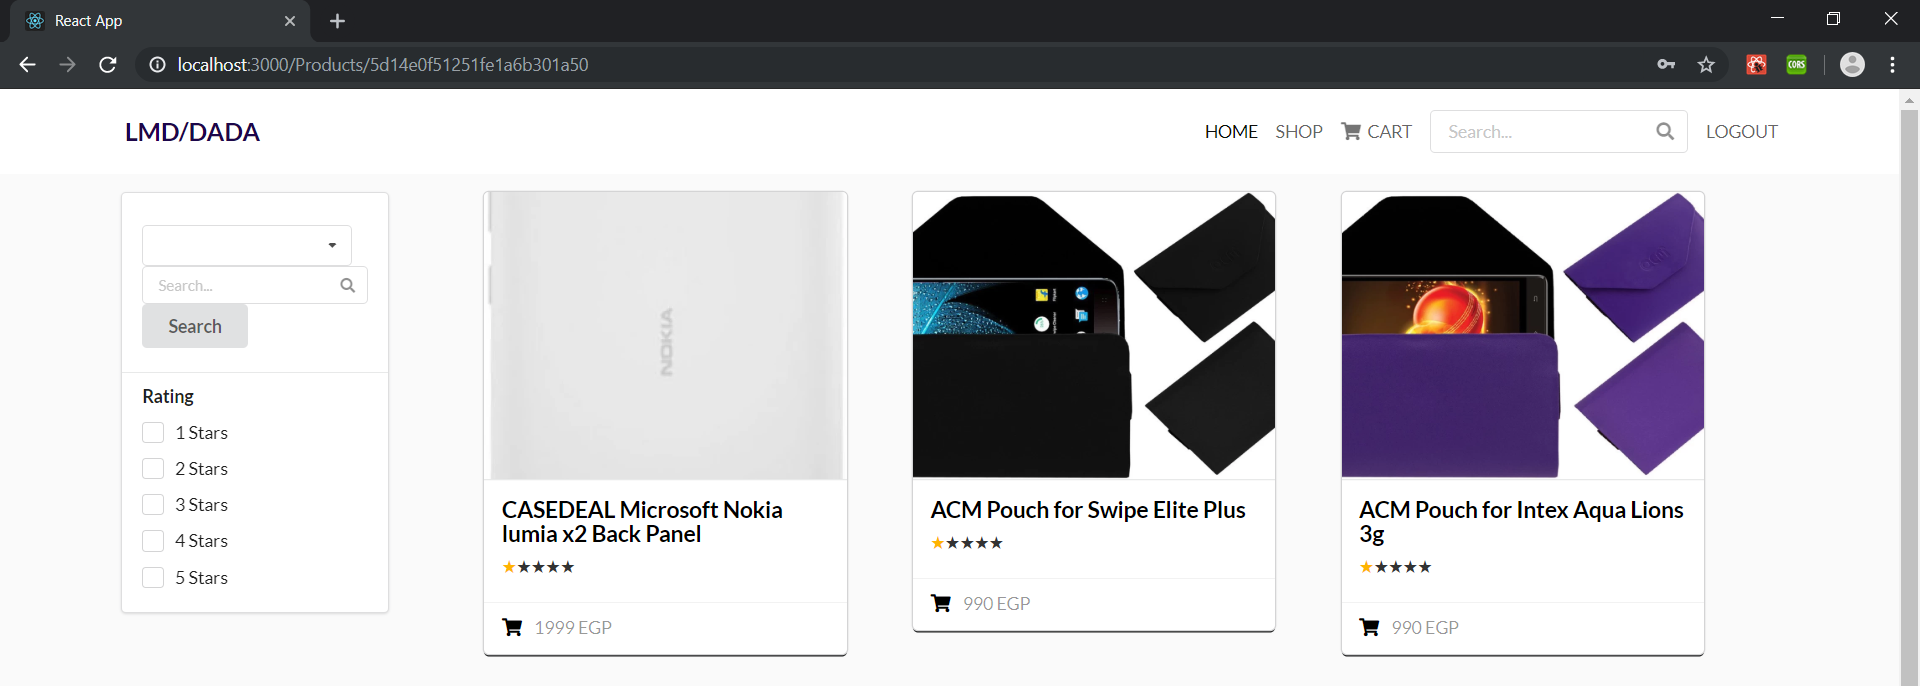
\includegraphics[width=1\textwidth]{images/Software/products.PNG}%
     % you need to add the caption for the list of figures
    \caption[Website: Products Page]{Website: Products Page}\label{fig: products}%
  \end{figure}\newline
  
    \begin{figure}[htp]%
    \center%
    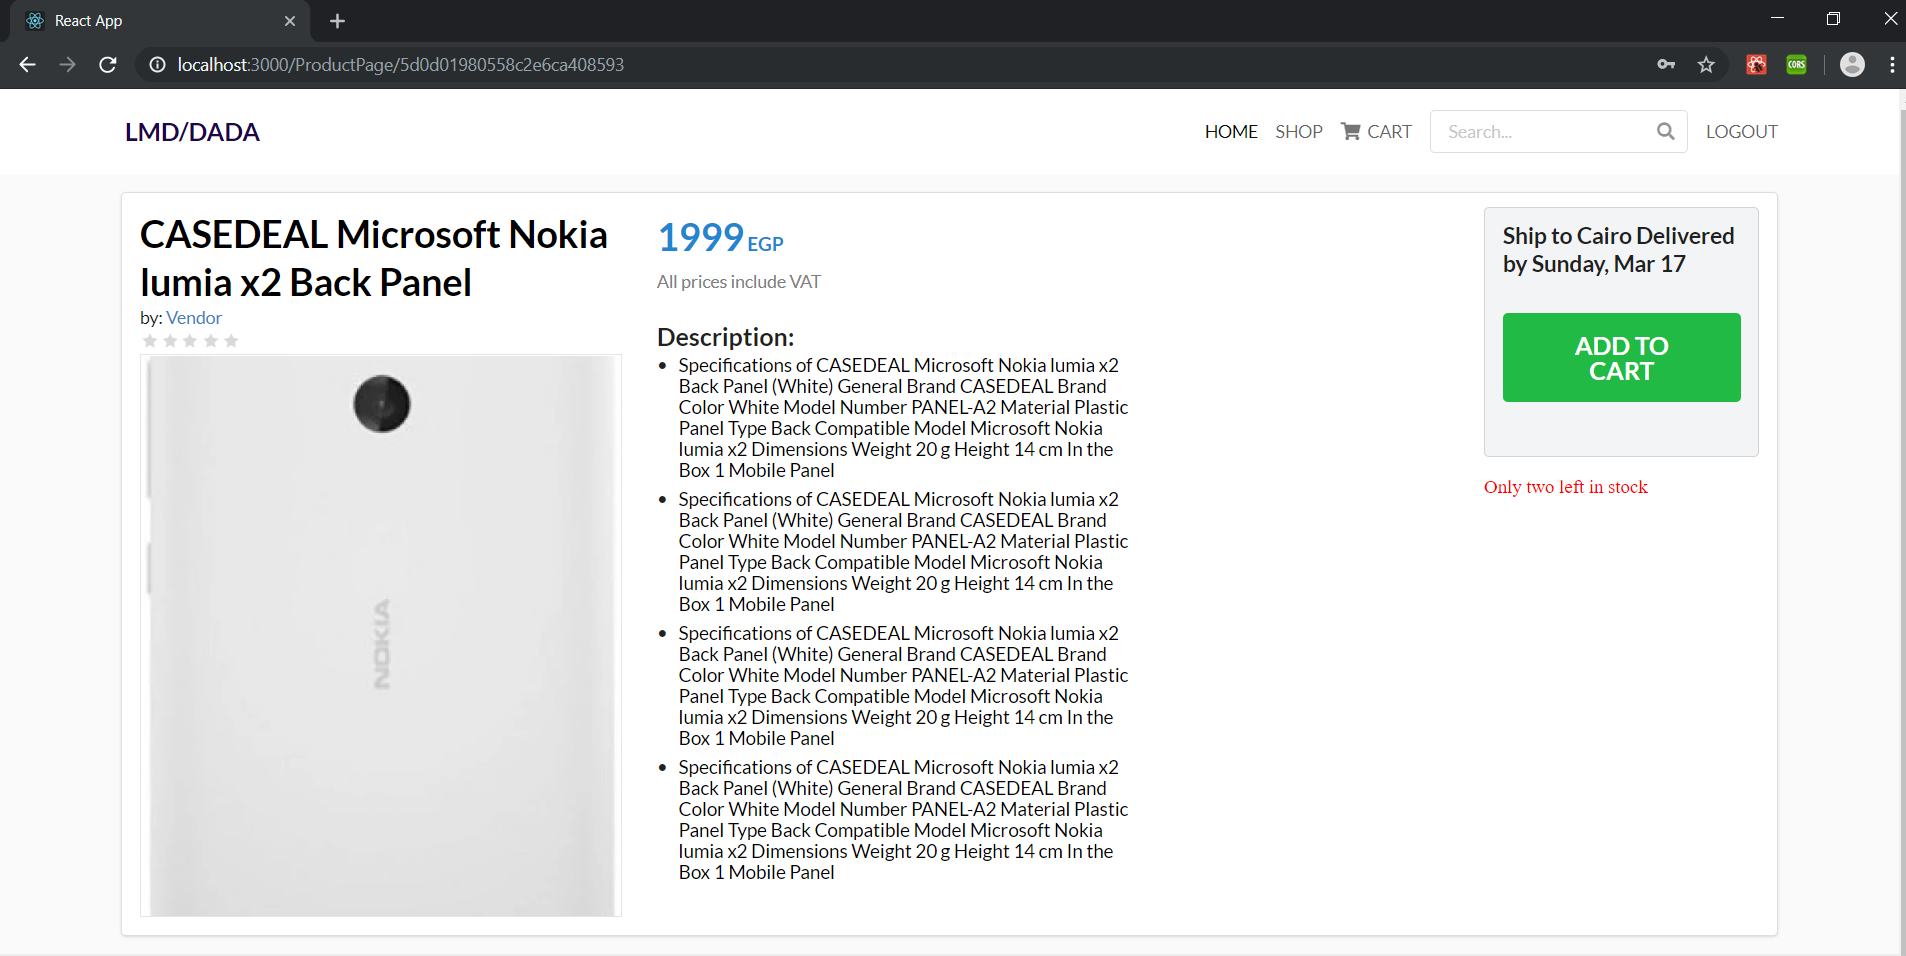
\includegraphics[width=1\textwidth]{images/Software/productPage.PNG}%
     % you need to add the caption for the list of figures
    \caption[Website: product Page]{Product Page}\label{fig: product Page}%
  \end{figure}\newpage
  

In Figure \ref{fig: cart} each user has its own cart with different elements to buy the “proceed to check out” button redirects the user to Stripe component as shown in figure  \ref{fig: payment} that access his location and visa card to continue to checkout.
Stripe is an American technology company its software allows individuals and businesses to make and receive payments over the Internet. Stripe provides the technical, fraud prevention, and banking infrastructure required to operate online payment systems \cite{Stripe}.

\begin{figure}[htp]%
    \center%
    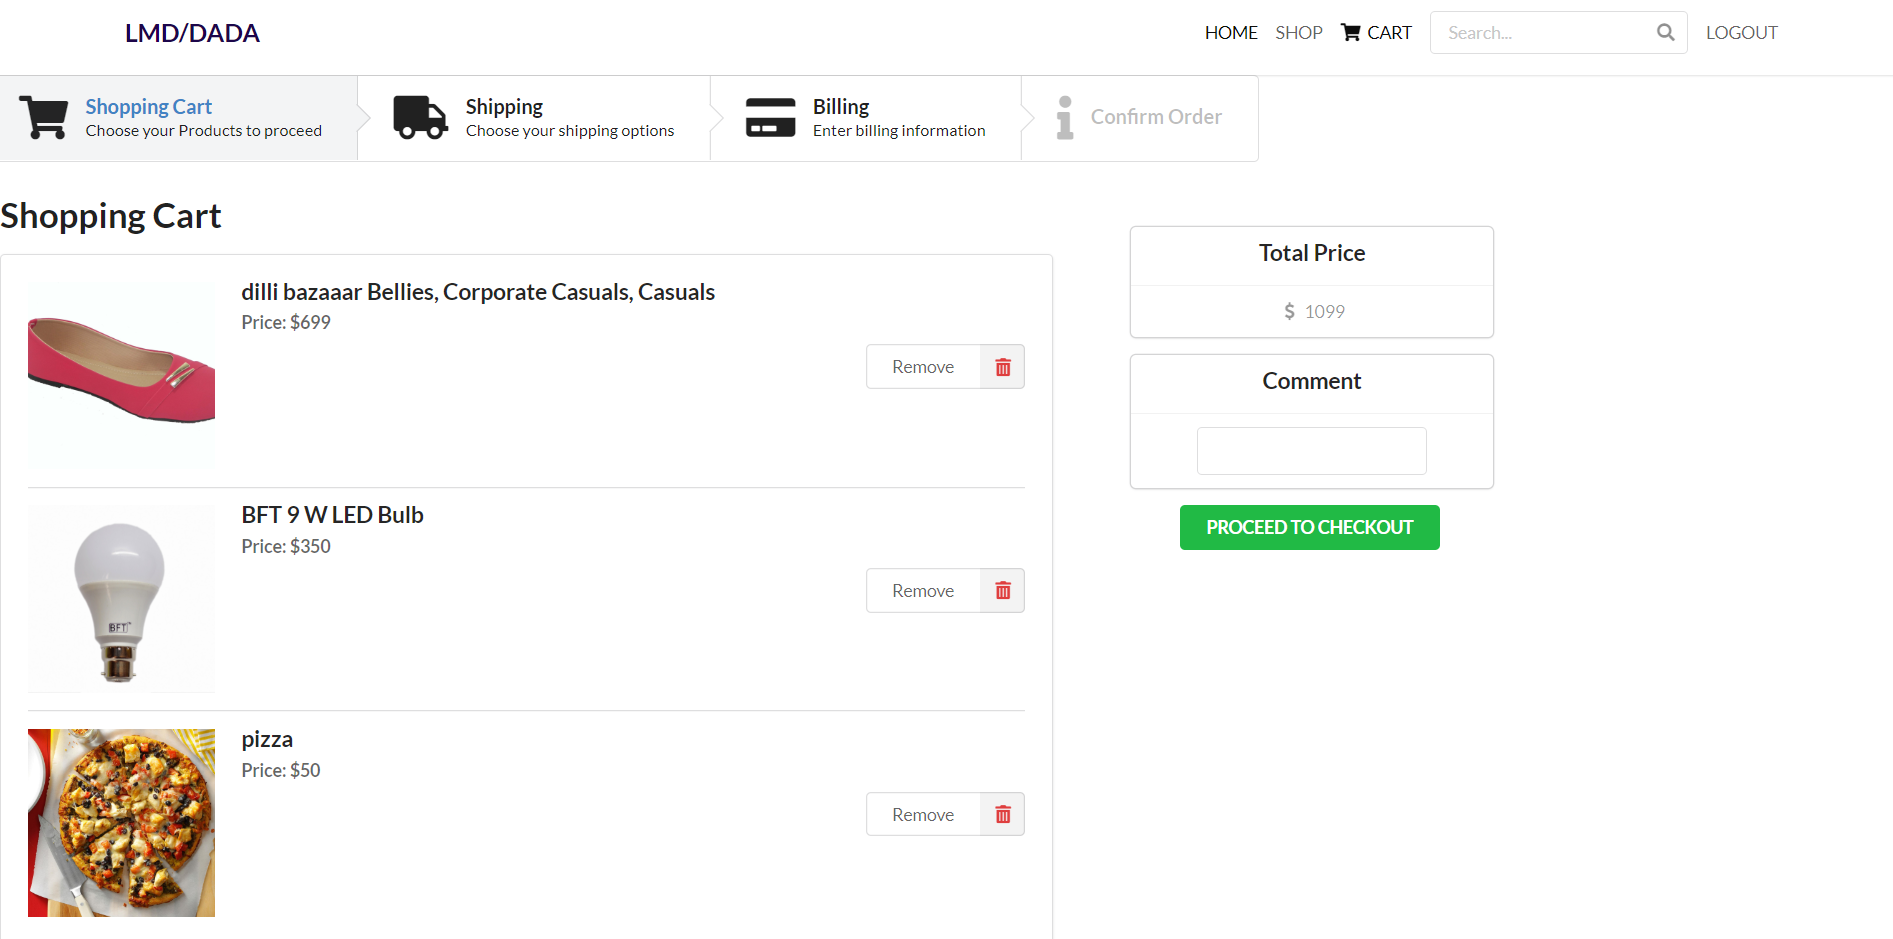
\includegraphics[width=1\textwidth]{images/Software/cart.PNG}%
     % you need to add the caption for the list of figures
    \caption[Website: Cart Page]{Website: Cart Page}\label{fig: cart}%
  \end{figure}
  
   \begin{figure}[htp]%
    \center%
    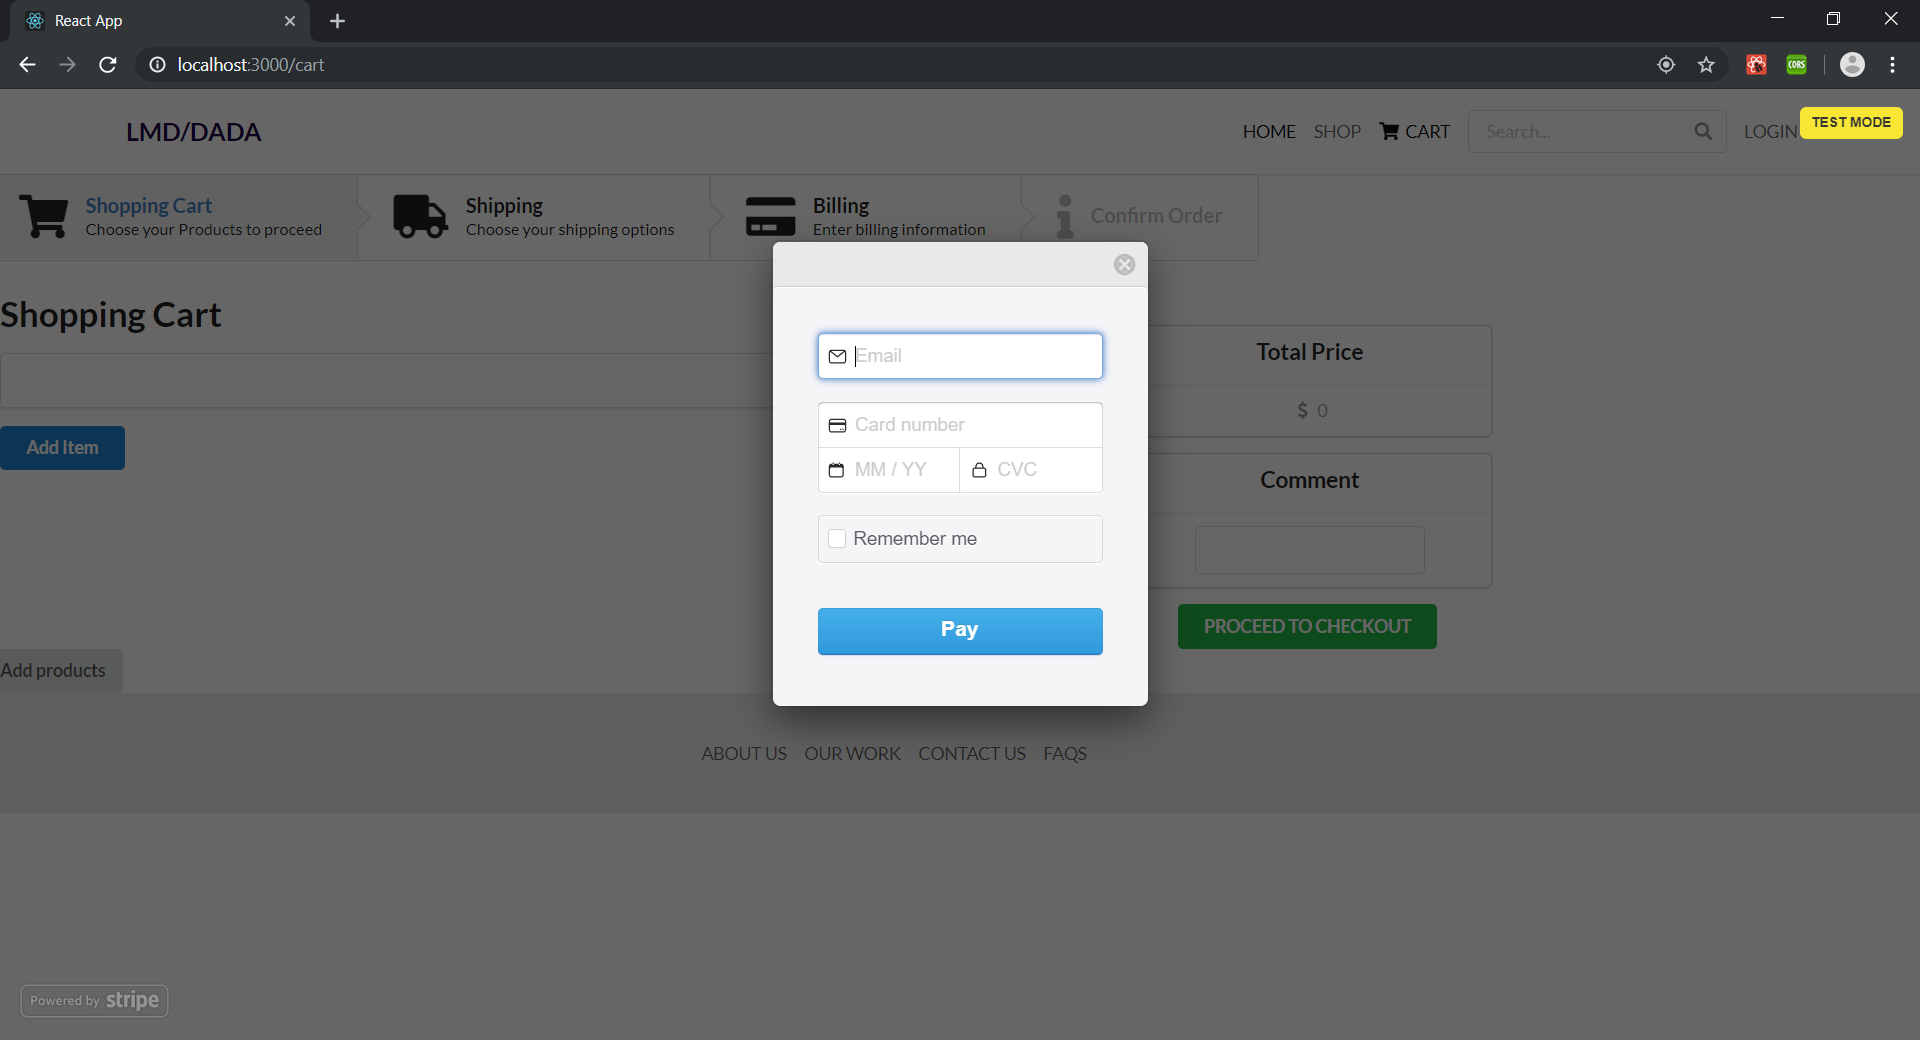
\includegraphics[width=1\textwidth]{images/Software/payment.PNG}%
     % you need to add the caption for the list of figures
    \caption[Website: Payment Page]{Website: Payment Page}\label{fig: payment}%
  \end{figure}\newpage

In figure \ref{fig: tracking} Tracking page is used to track the robot carrying the order with tracking password as shown in figure\ref{fig:trackPas}.
  \begin{figure}[htp]%
    \center%
    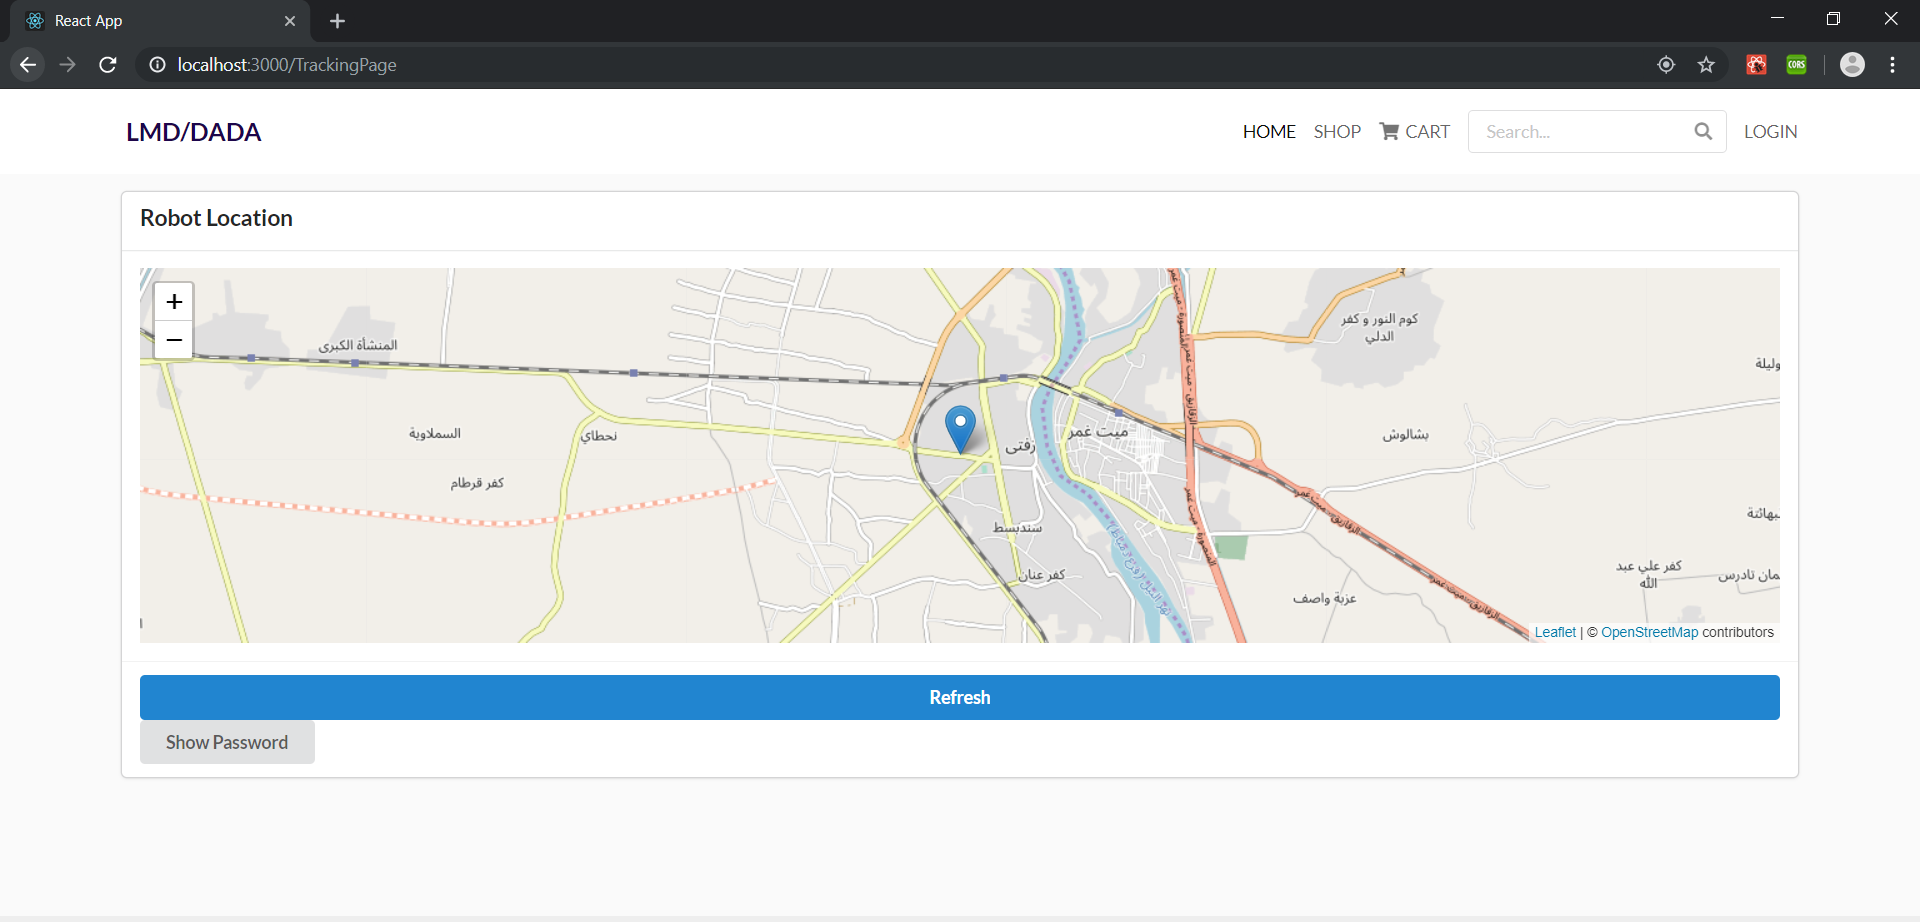
\includegraphics[width=1\textwidth]{images/Software/tracking.PNG}%
     % you need to add the caption for the list of figures
    \caption[Website: Tracking Page]{Tracking Page}\label{fig: tracking}%
  \end{figure}
  
    \begin{figure}[htp]%
    \center%
    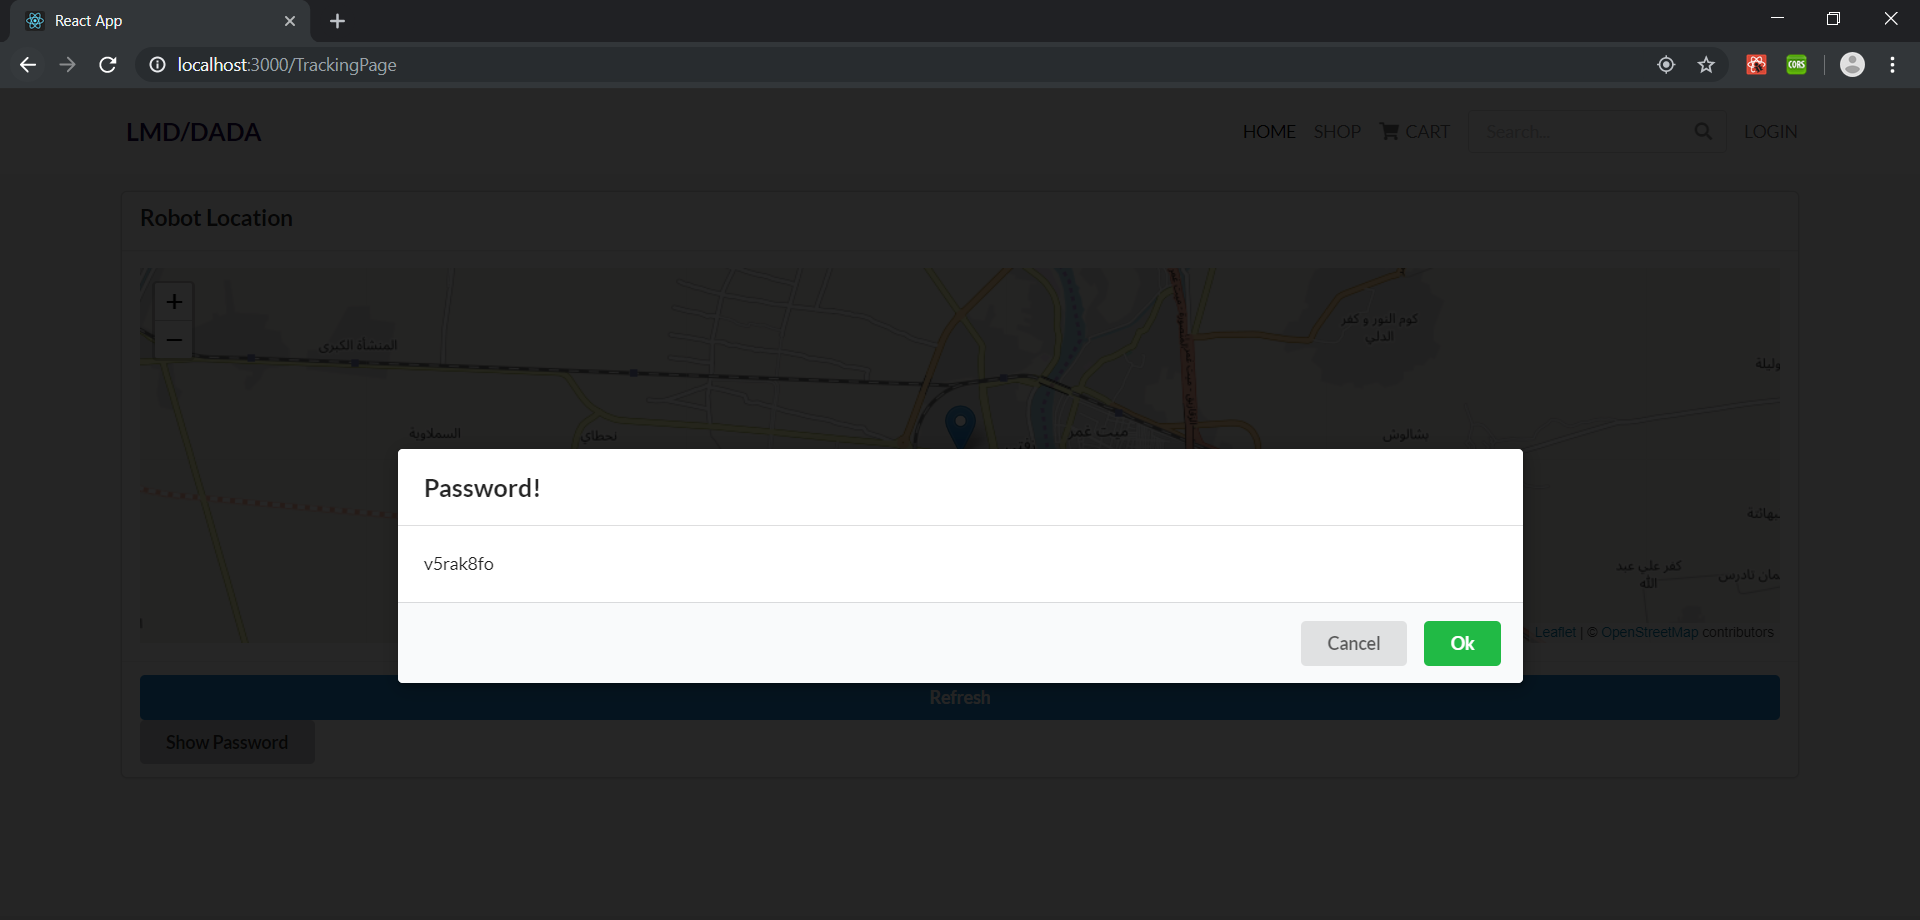
\includegraphics[width=1\textwidth]{images/Software/trackingPassword.PNG}%
     % you need to add the caption for the list of figures
    \caption[Website: Tracking Password Page]{ Tracking Password Page}\label{fig:trackPas}%
  \end{figure}
  
Also the vendor has its own page to add his products as shown in figure \ref{fig: add Product}.
  \begin{figure}[htp]%
    \center%
    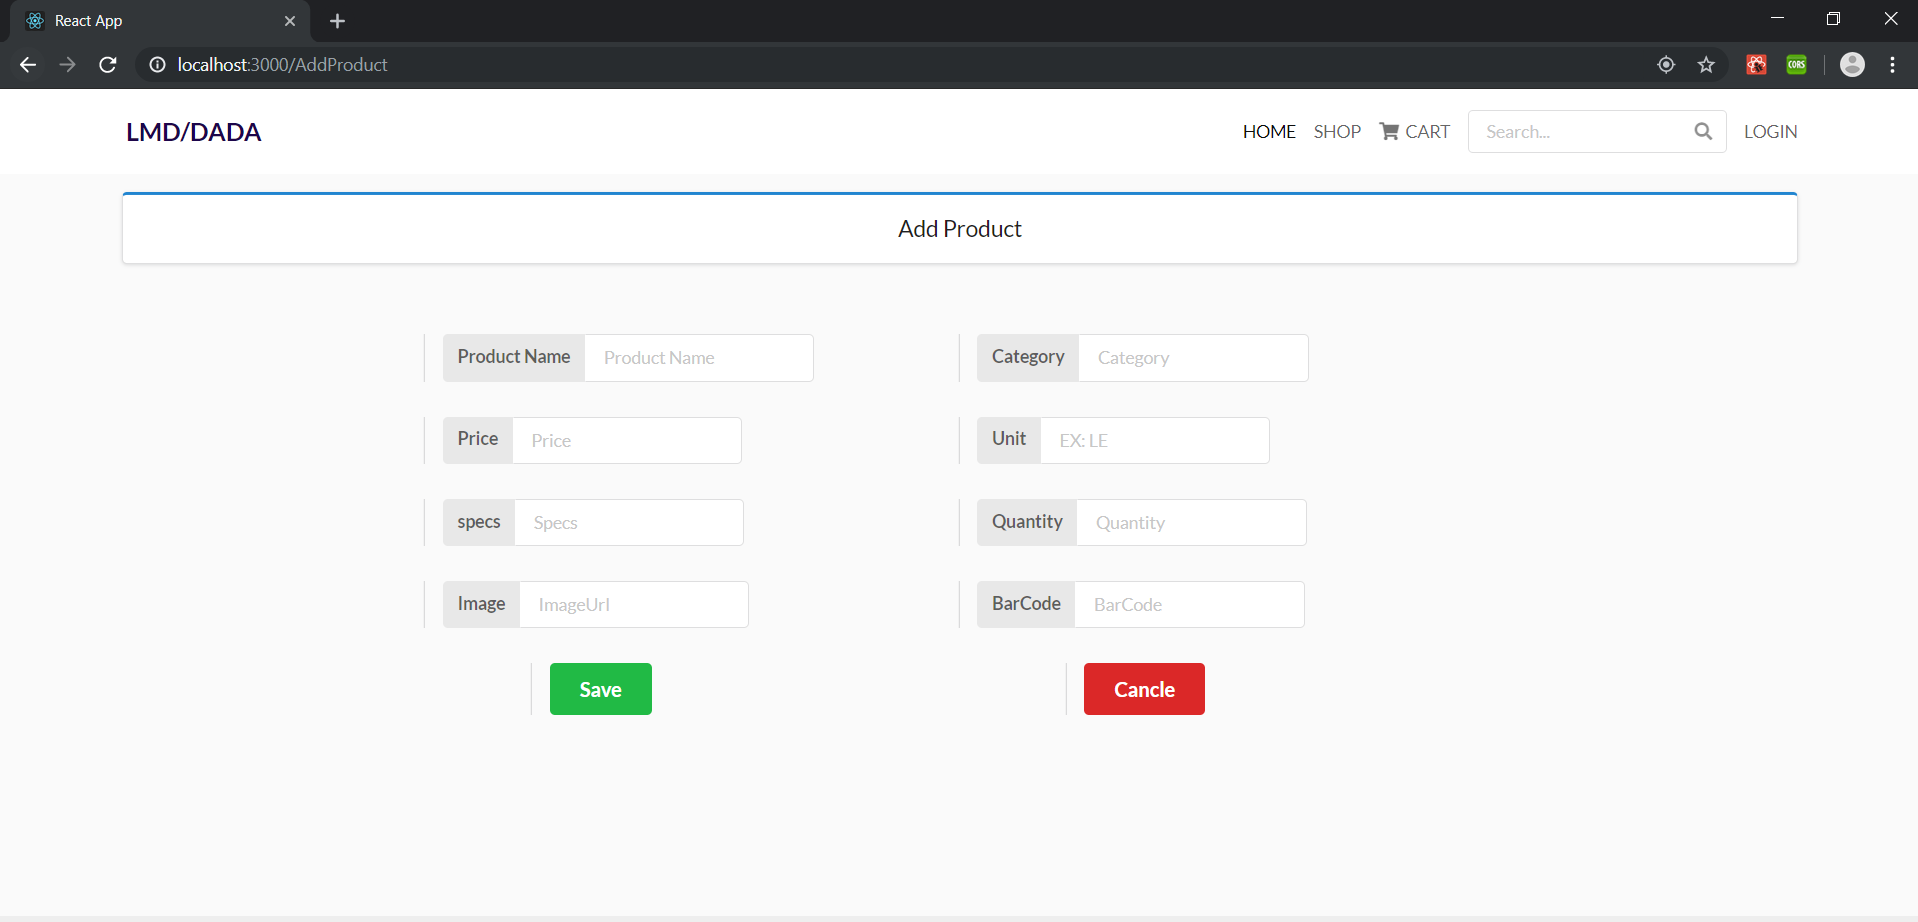
\includegraphics[width=1\textwidth]{images/Software/addProduct.PNG}%
     % you need to add the caption for the list of figures
    \caption[Website: Add Product Page]{Website: Add Product Page}\label{fig: add Product}%
  \end{figure} \newpage
  
At last, we have our page that defines the scope of the project and the team members as shown in figure \ref{fig: about1}
  \begin{figure}[htp]%
    \center%
    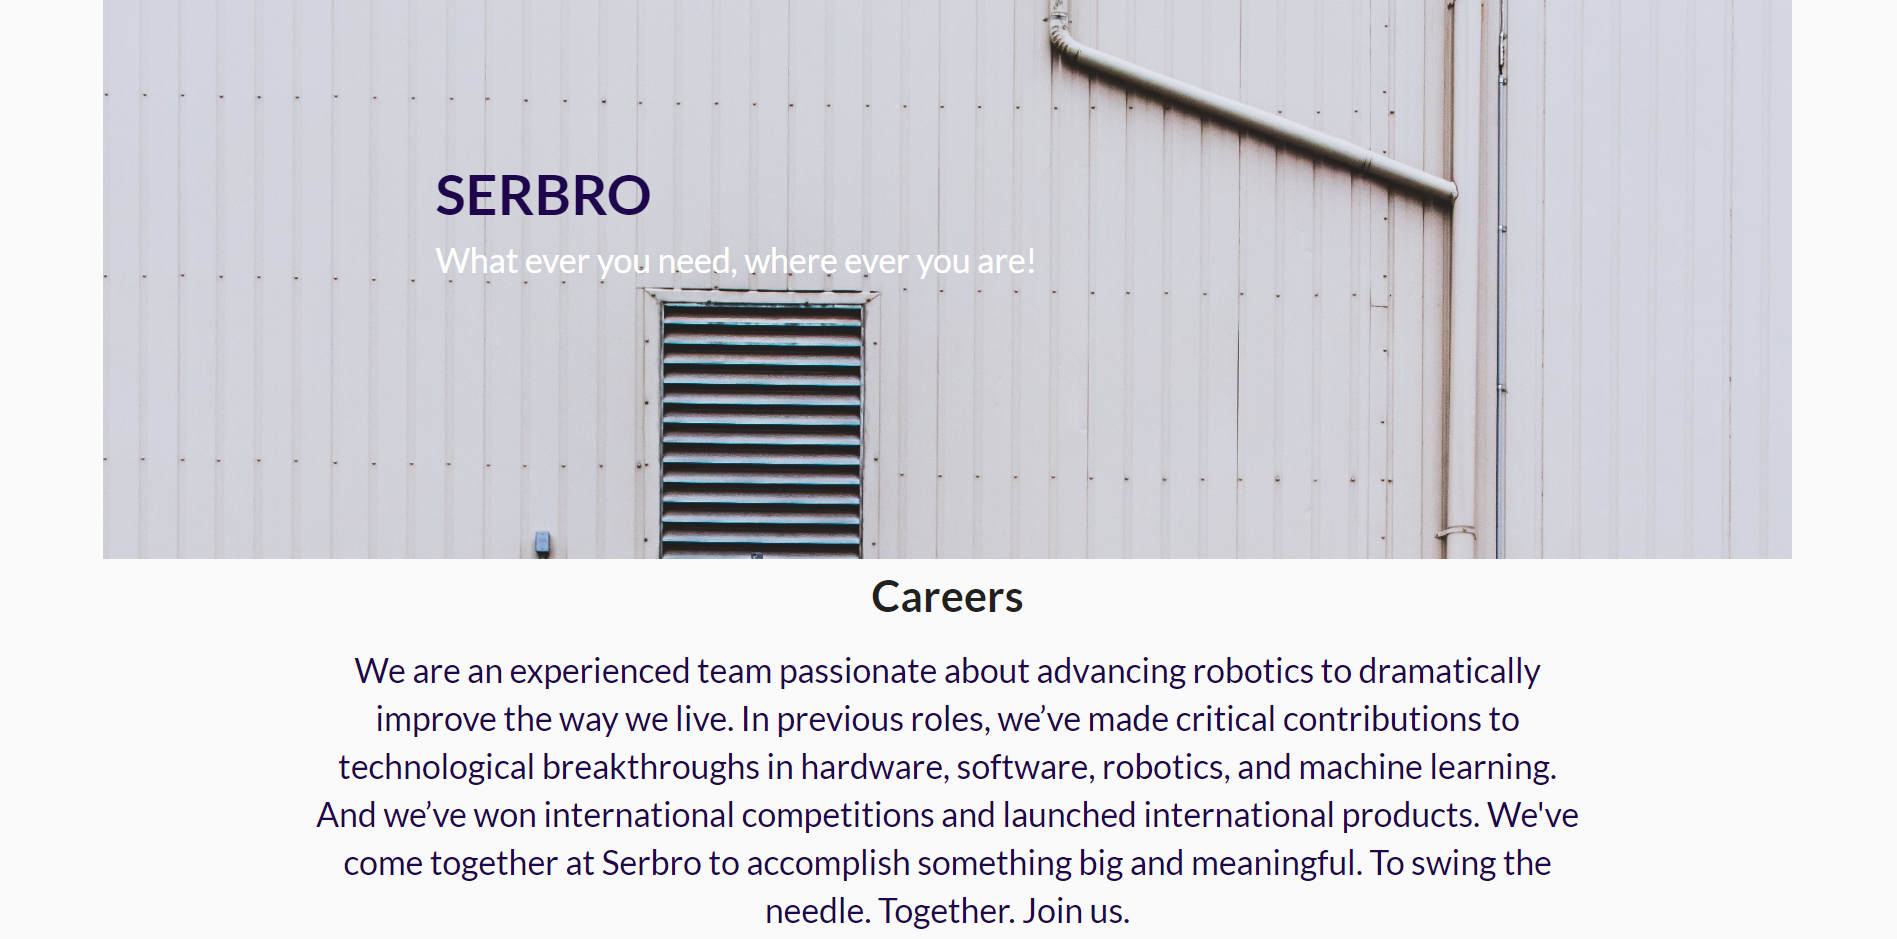
\includegraphics[width=1\textwidth]{images/Software/about1.PNG}%
     % you need to add the caption for the list of figures
    \caption[Website: About Page (i)]{Website:  About Page (i)}\label{fig: about1}%
  \end{figure}
   \begin{figure}[htp]%
    \center%
    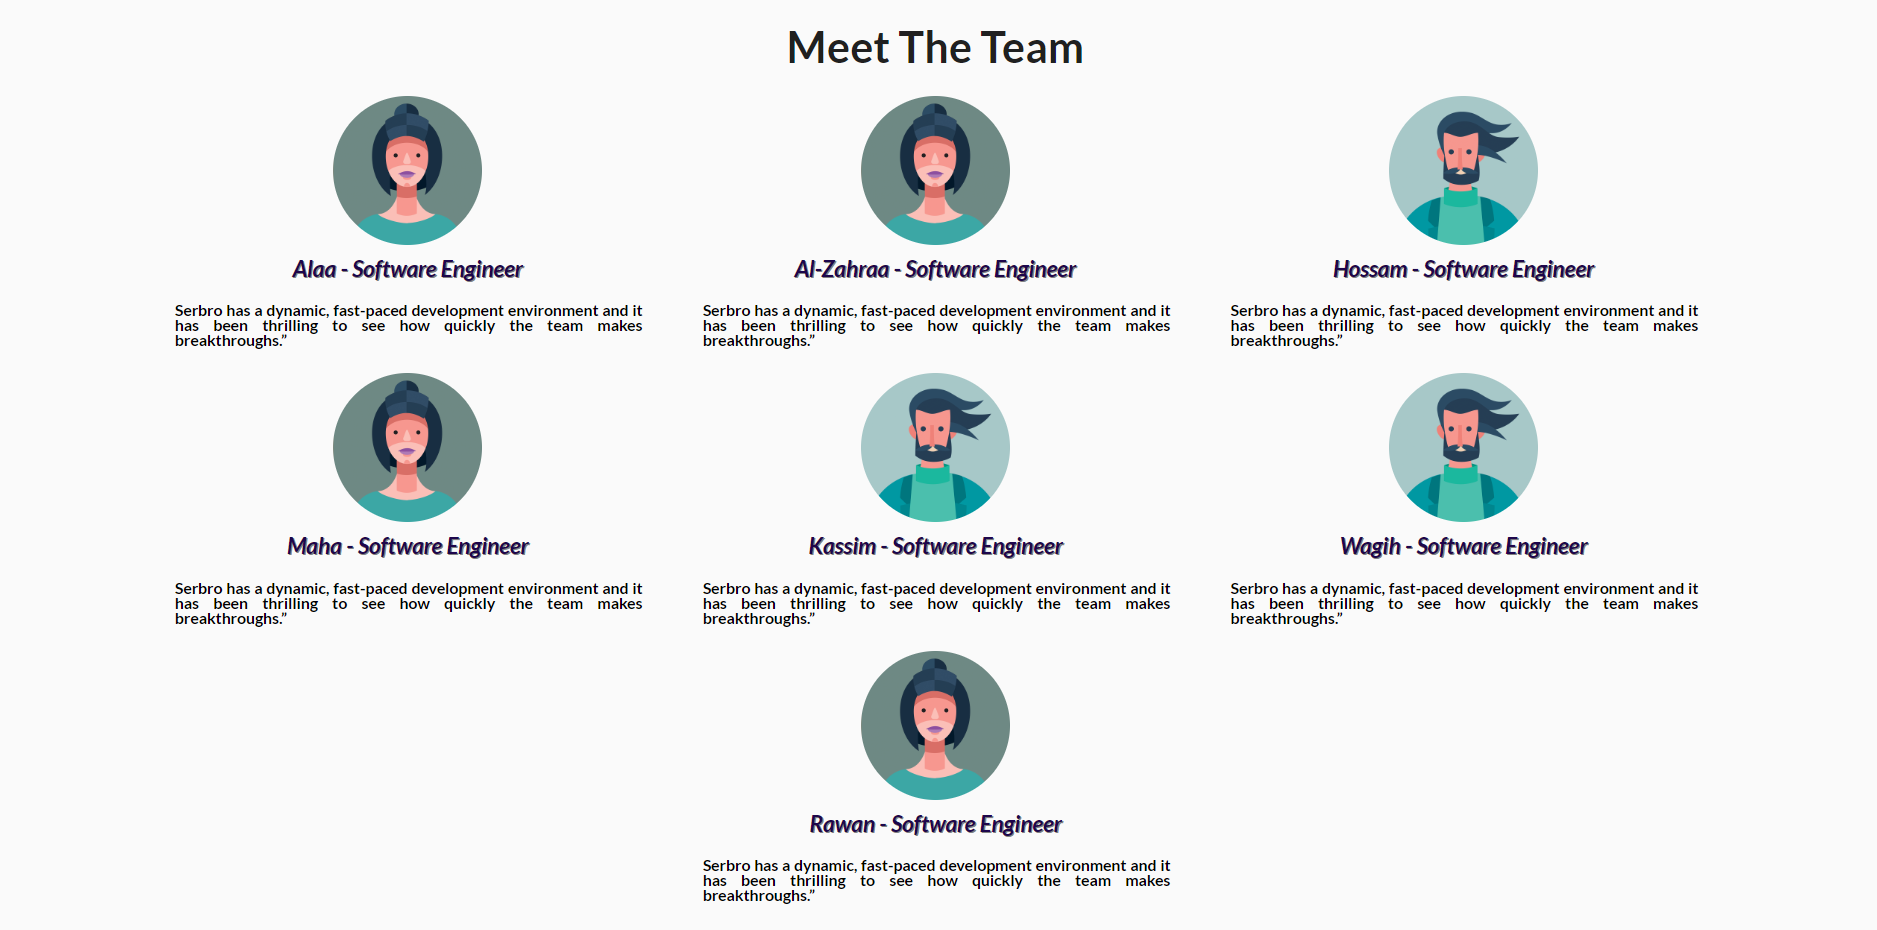
\includegraphics[width=1\textwidth]{images/Software/about2.PNG}%
     % you need to add the caption for the list of figures
    \caption[Website: About Page (ii)]{Website:  About Page (ii)}\label{fig: about2}%
  \end{figure}
\section{Mobile Front-End}
\hspace{2cm}We use React  which is a JavaScript framework for writing real, natively rendering mobile applications for iOS and Android. It’s based on React, Facebook’s JavaScript library for building user interfaces,but instead of targeting the browser, it targets mobile platforms.

Similar to React for the Web, React Native applications are written using a mixture of JavaScript and XML-esque markup, known as JSX. Then, under the hood, the React Native “bridge” invokes the native rendering APIs in Objective-C (for iOS) or Java (for Android). Thus, your application will render using real mobile UI components, not webviews, and will look and feel like any other mobile application. React Native also exposes JavaScript interfaces for platform APIs, so your React Native apps can access platform features like the phone camera, or the user’s location \cite{React-native}.\newpage

\textbf{Mobile Screens}:
\newline
 In figure \ref{fig: homescreen} main page contains our logo and top categories such as (Food, Health and Clothes), the user can access the shop or choose his favourite category.

\begin{figure}[htp]%
    \center%
    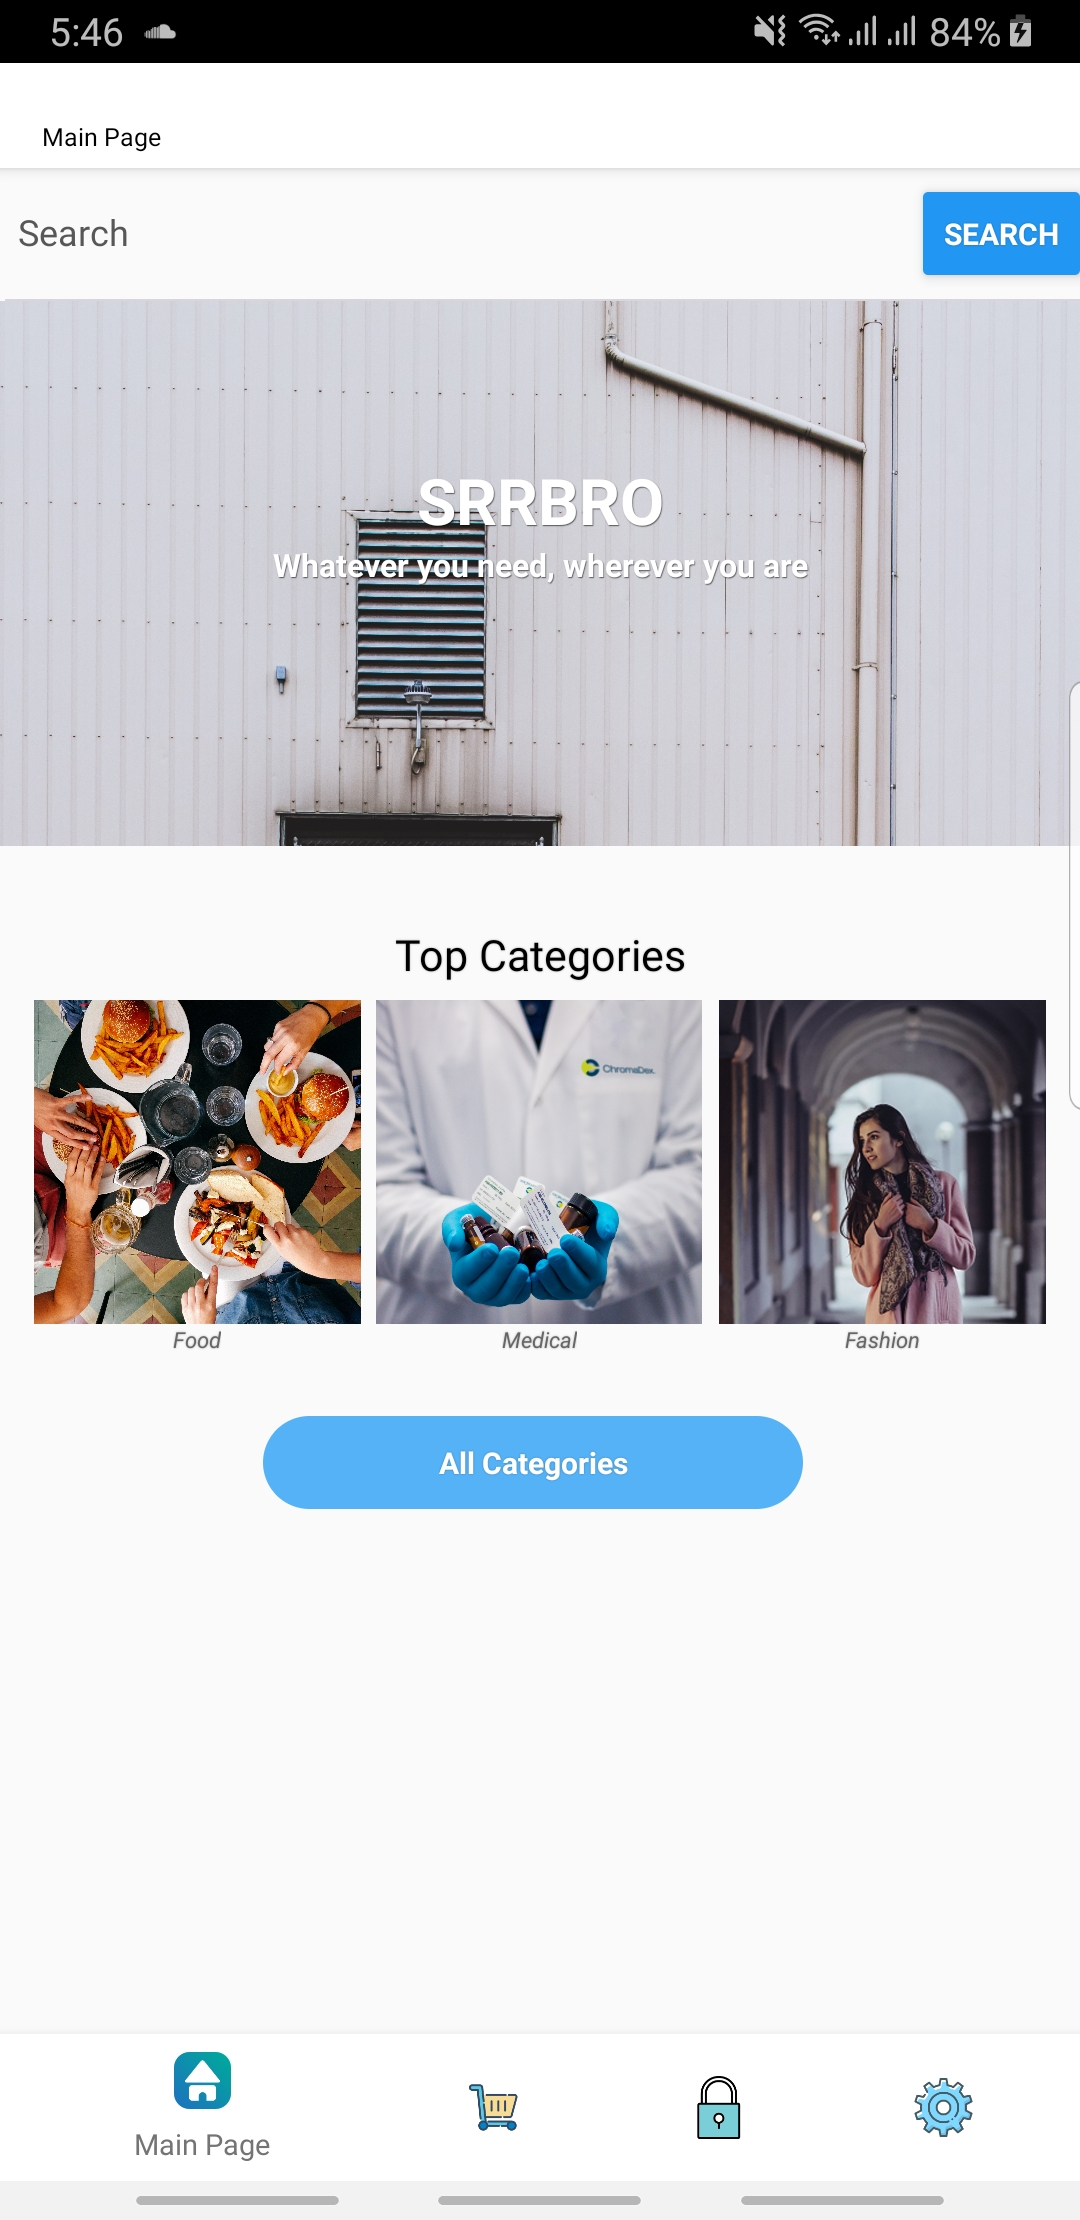
\includegraphics[width=0.52\textwidth]{images/Software/Mainscreen.jpg}%
     % you need to add the caption for the list of figures
    \caption[Mobile Application: Home Screen]{Mobile Application: Home Screen}\label{fig: homescreen}%
  \end{figure}
  
  
In Figure \ref{fig: singin} a login Screen to enter the email and password also checks that the user must be authorized.it also contain sing up page if the user doesn't have account on our system.

\begin{figure}[htp]%
    \center%
    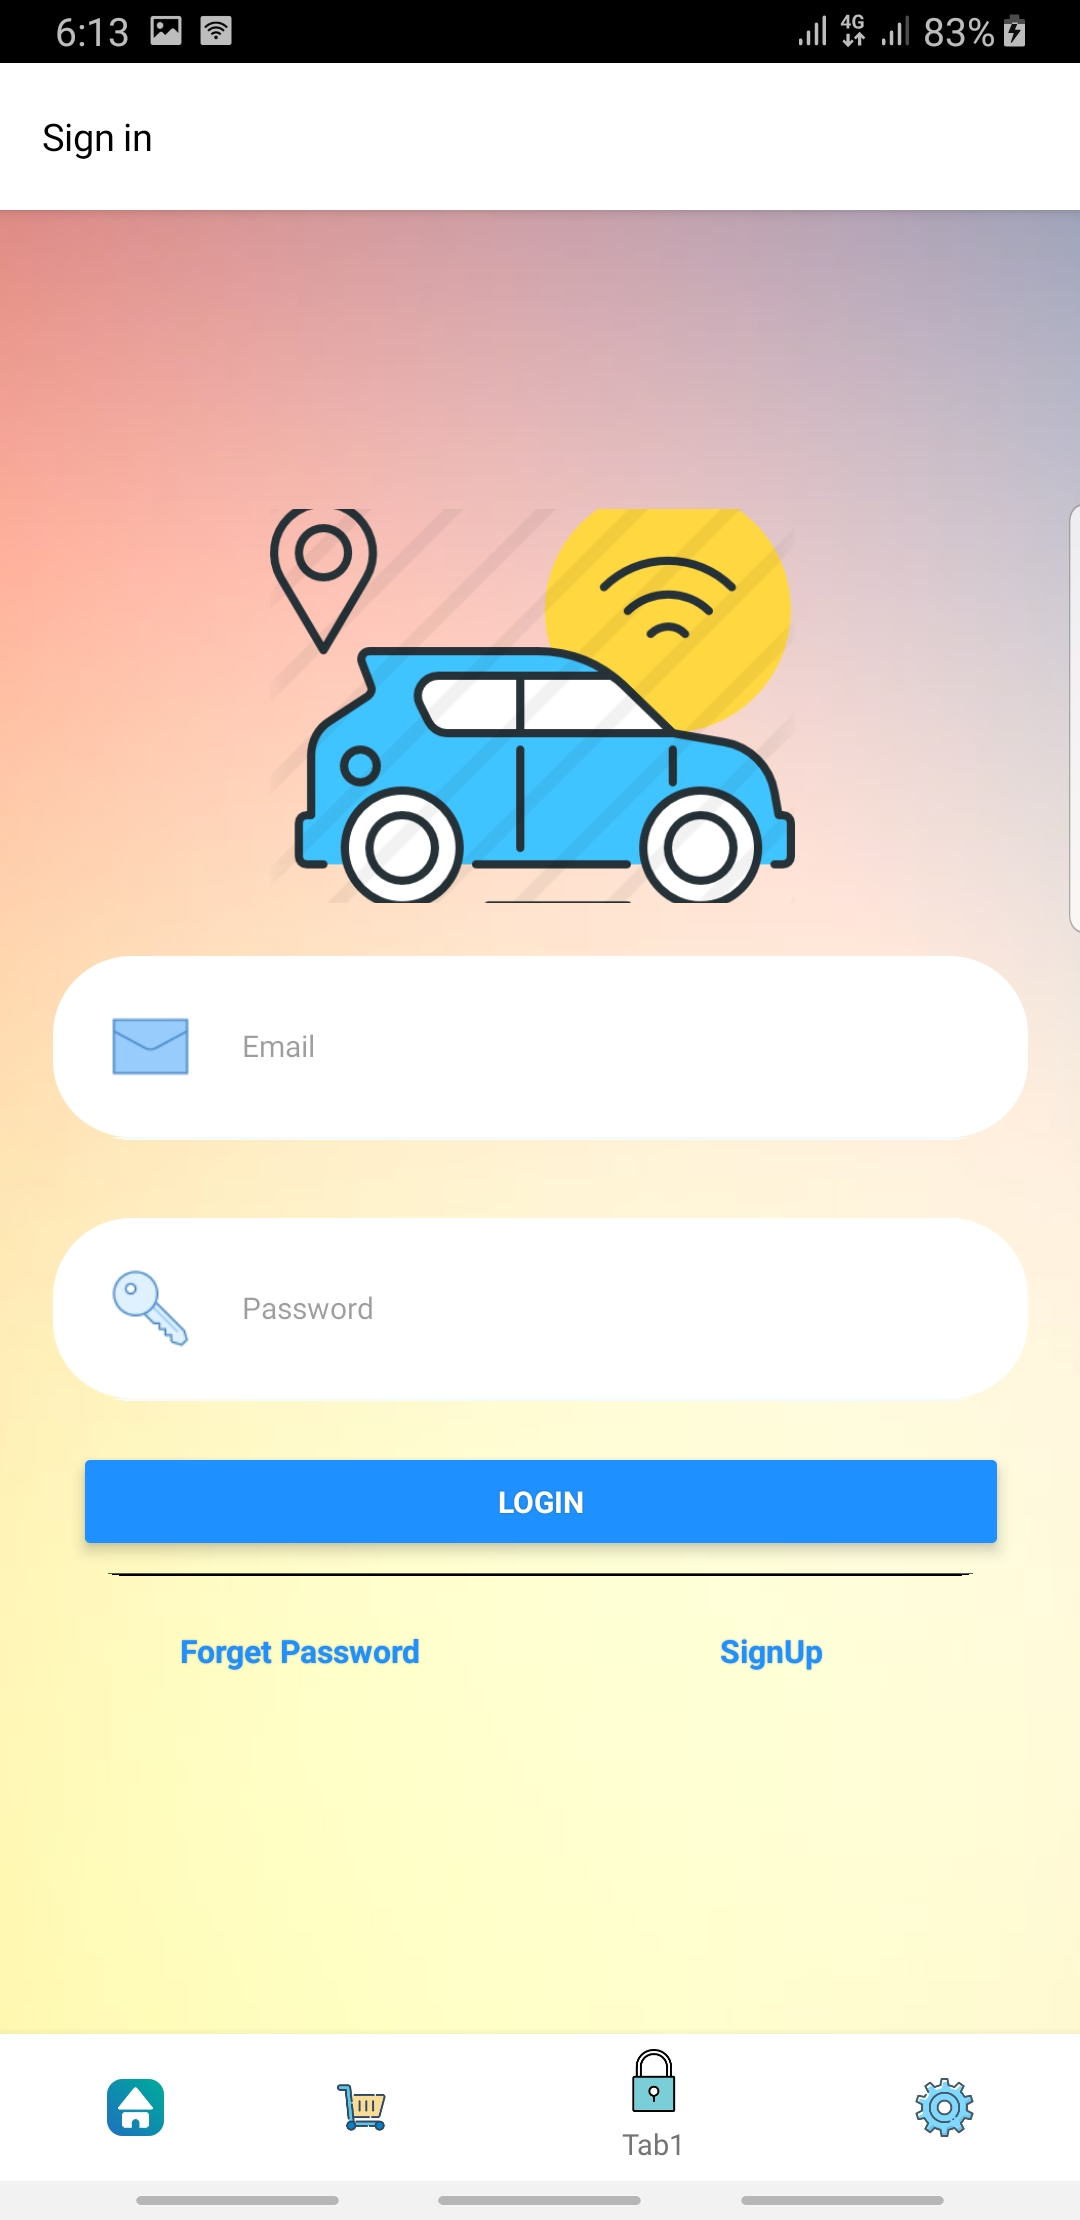
\includegraphics[width=0.52\textwidth]{images/Software/signin.jpg}%
     % you need to add the caption for the list of figures
    \caption[Mobile Application: Login Screen]{Mobile Application: Login Screen}\label{fig: singin}%
  \end{figure}
\newpage  


In Figure \ref{fig: singup} a Sing Up to register new user in our system.
\begin{figure}[htp]%
    \center%
    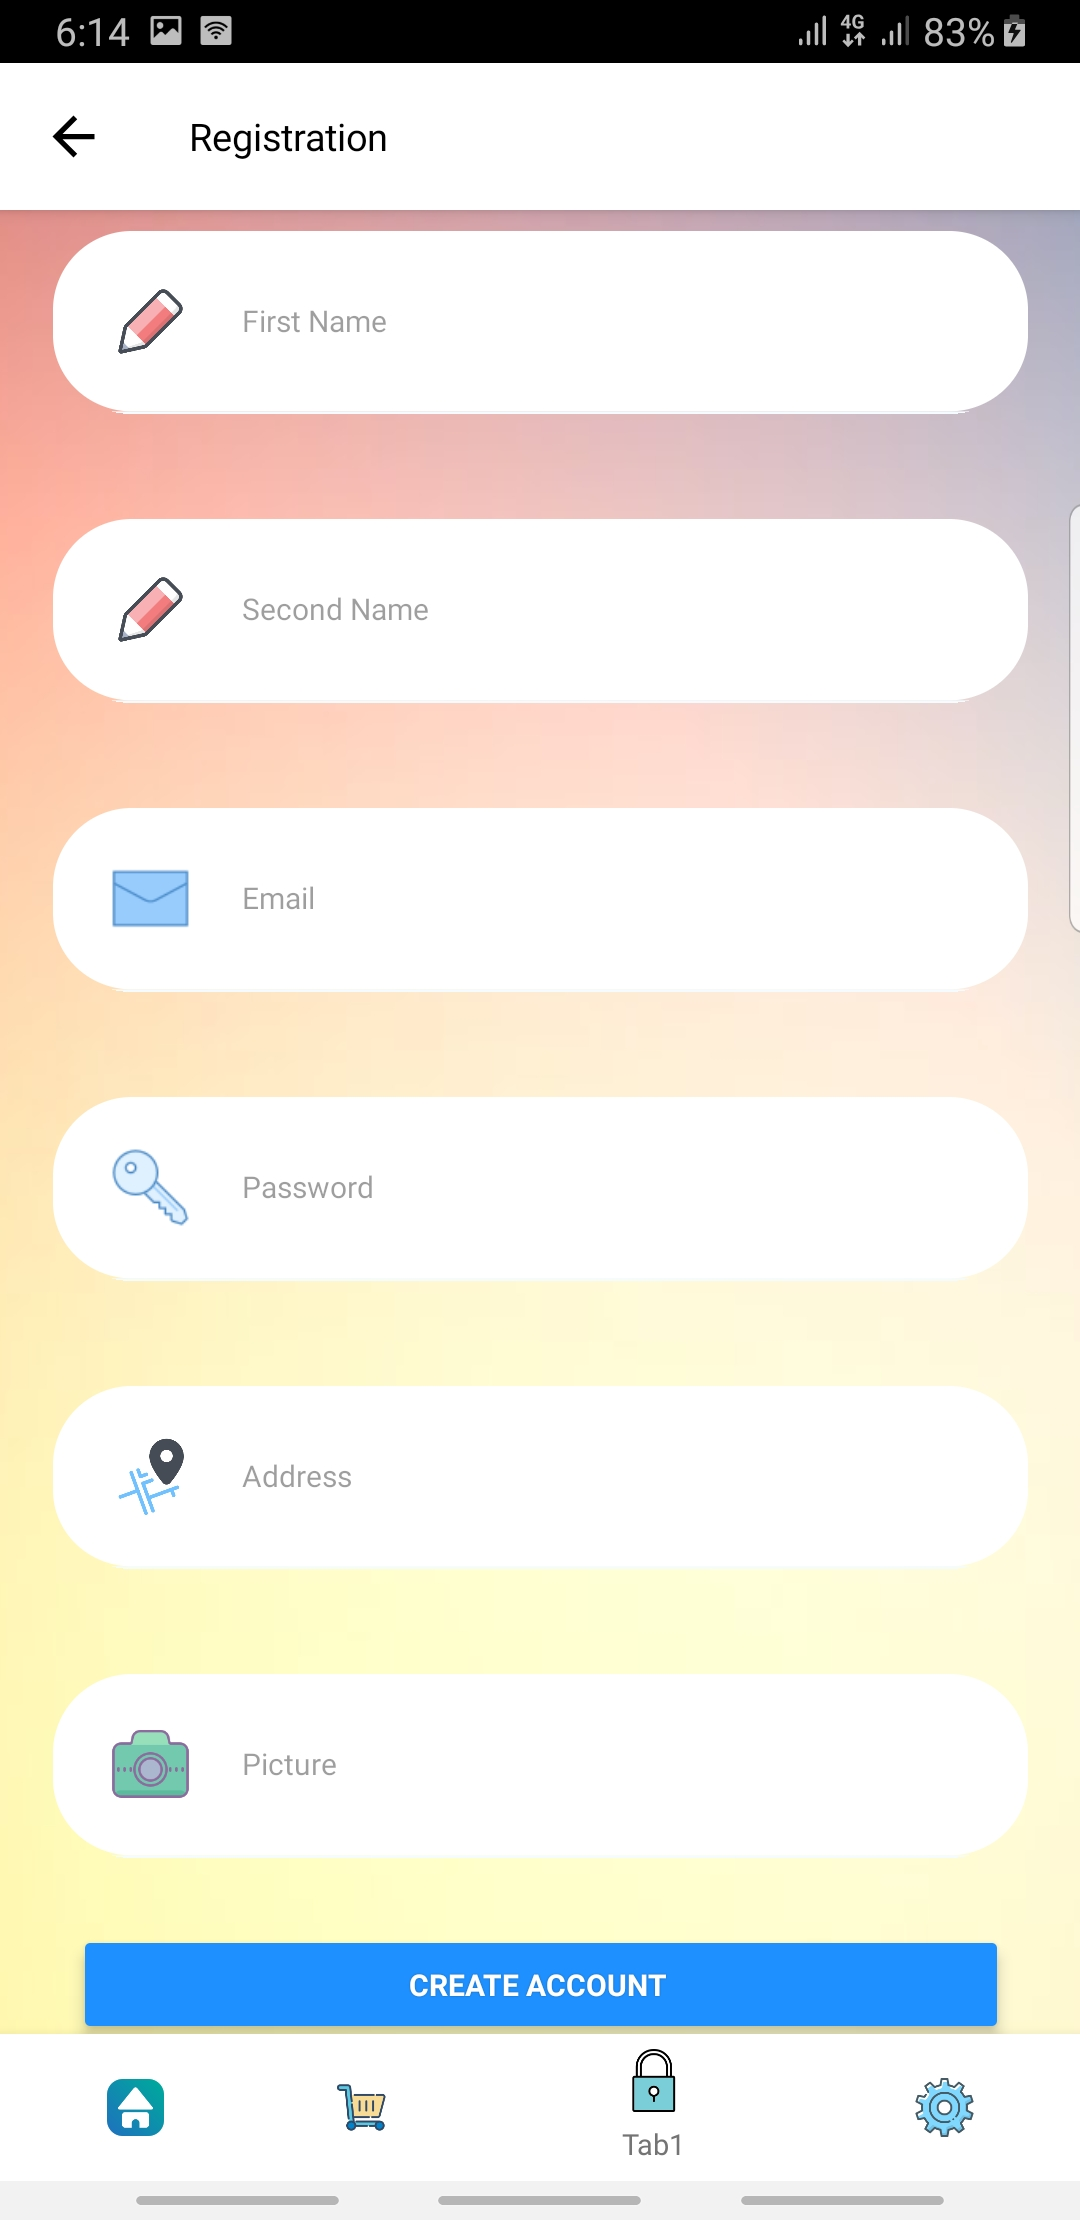
\includegraphics[width=0.5\textwidth]{images/Software/signup.jpg}%
     % you need to add the caption for the list of figures
    \caption[Mobile Application: Sing up Screen]{Mobile Application: Sing up Screen}\label{fig: singup}%
  \end{figure}
\newpage


In Figure \ref{fig: shop} shop Screen has our vendors in the system.
  \begin{figure}[htp]%
    \center%
    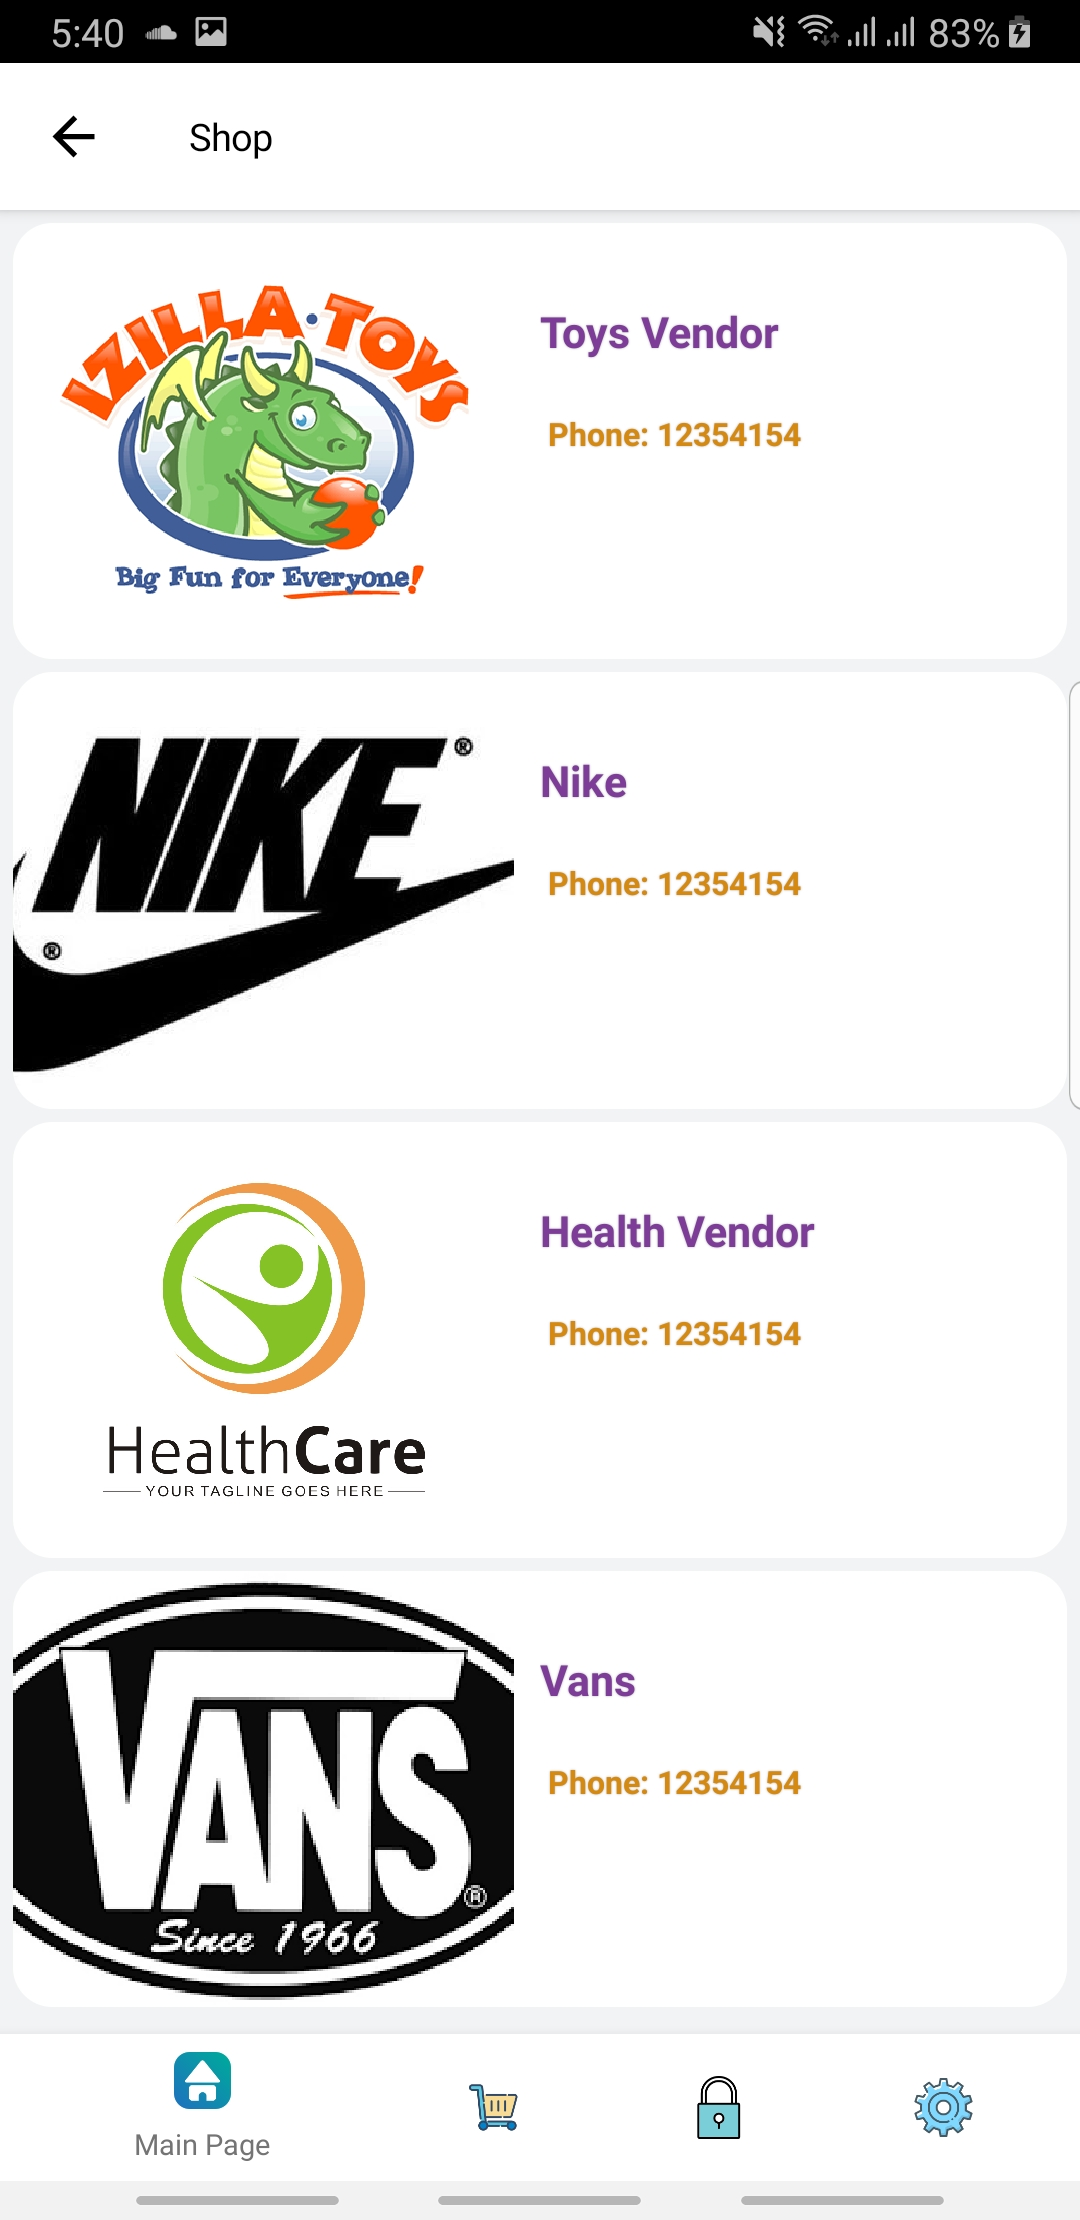
\includegraphics[width=0.5\textwidth]{images/Software/Shop.jpg}%
     % you need to add the caption for the list of figures
    \caption[Mobile Application: Shop Screen]{Shop Screen}\label{fig: shop}%
  \end{figure} \newpage
  
 In figure \ref{fig: productsscreen} Each Vendors have their products with description provided it product page in figure \ref{fig: productPageScreen} , search and filter by category are available while browsing and from product page the user can add this product to his cart.
  
  \begin{figure}[htp]%
    \center%
    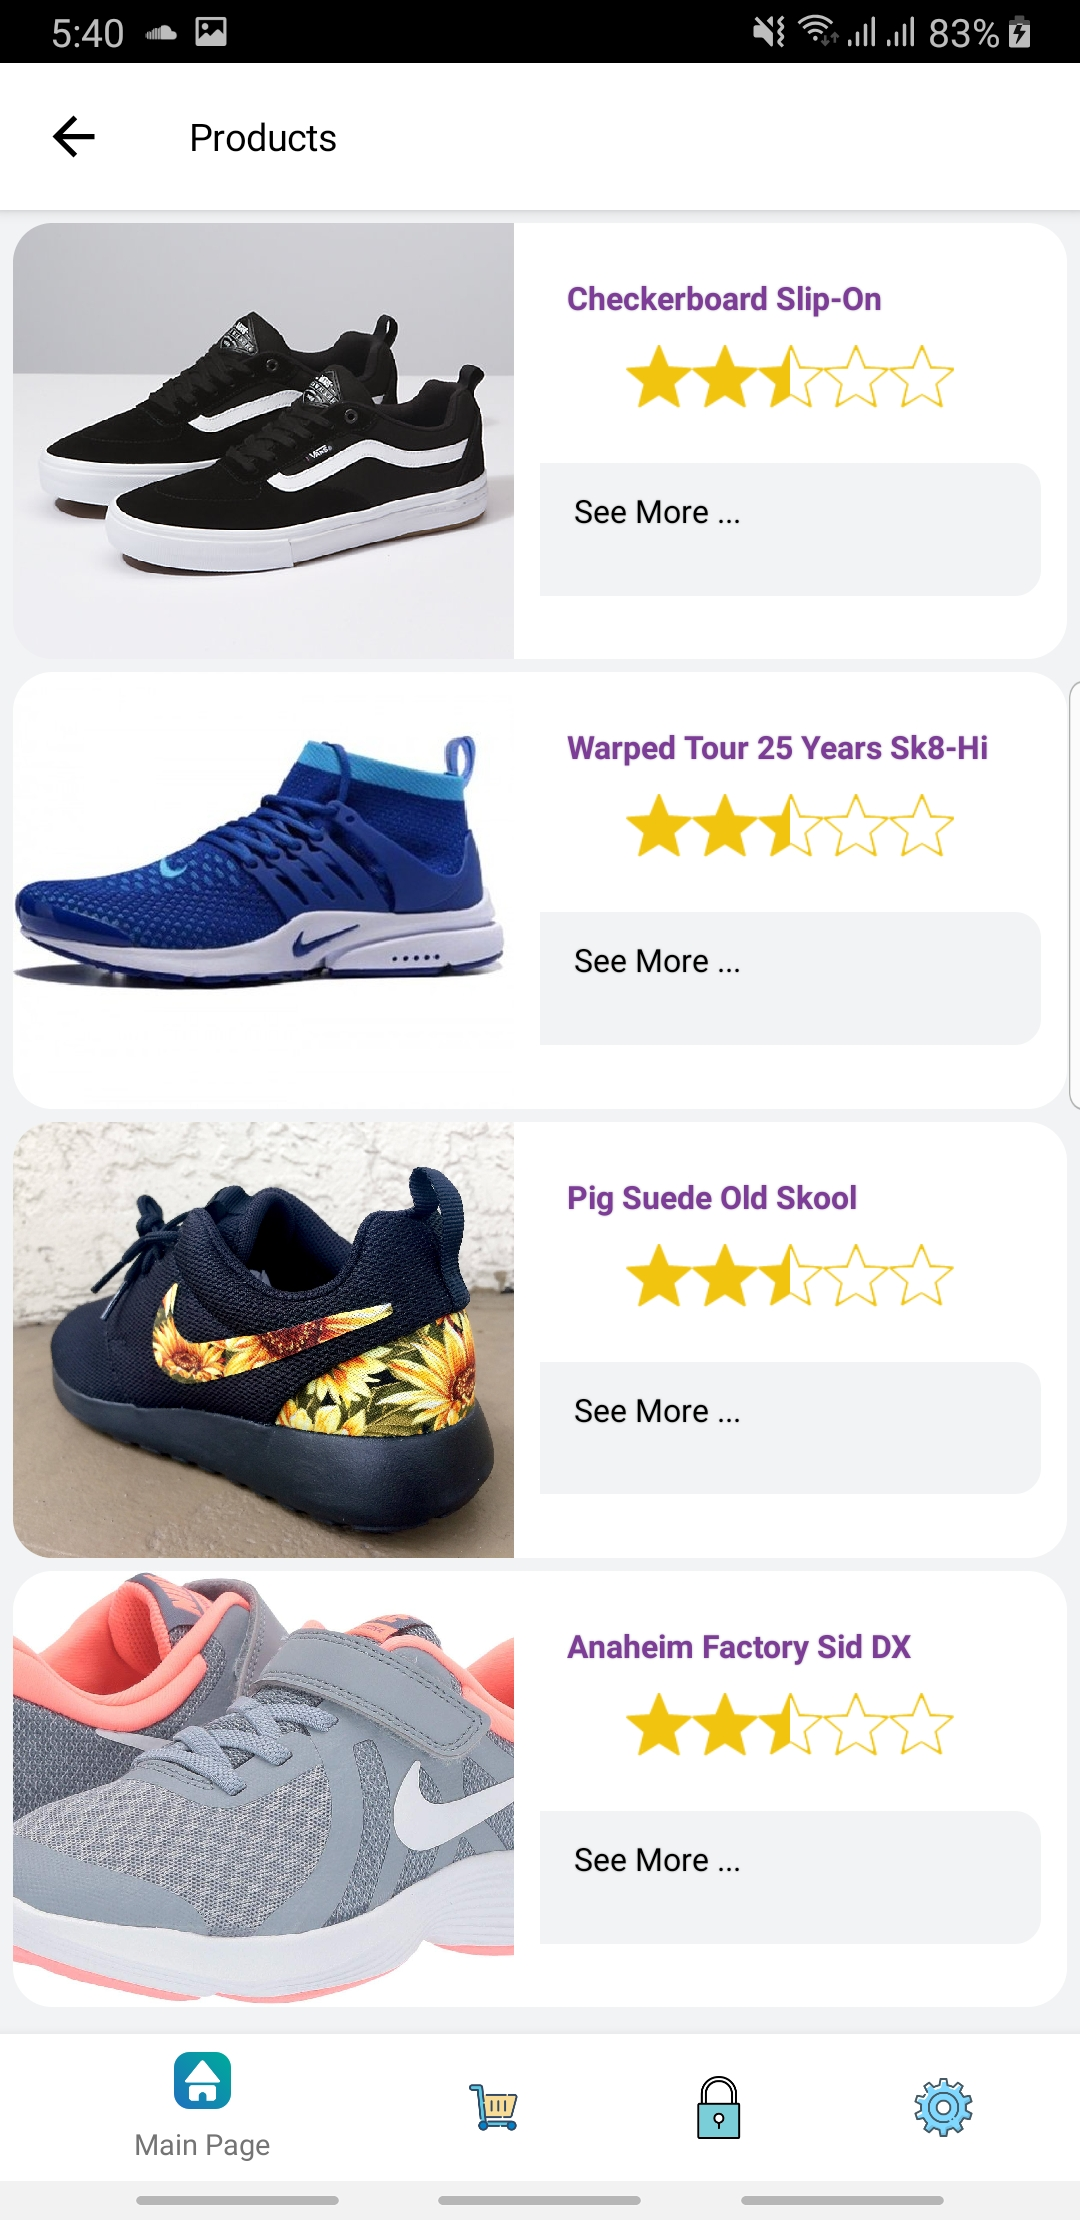
\includegraphics[width=0.5\textwidth]{images/Software/productsscreen.jpg}%
     % you need to add the caption for the list of figures
    \caption[Mobile Application:Products Screen]{Products Screen}\label{fig: productsscreen}%
  \end{figure}
  
    \begin{figure}[htp]%
    \center%
    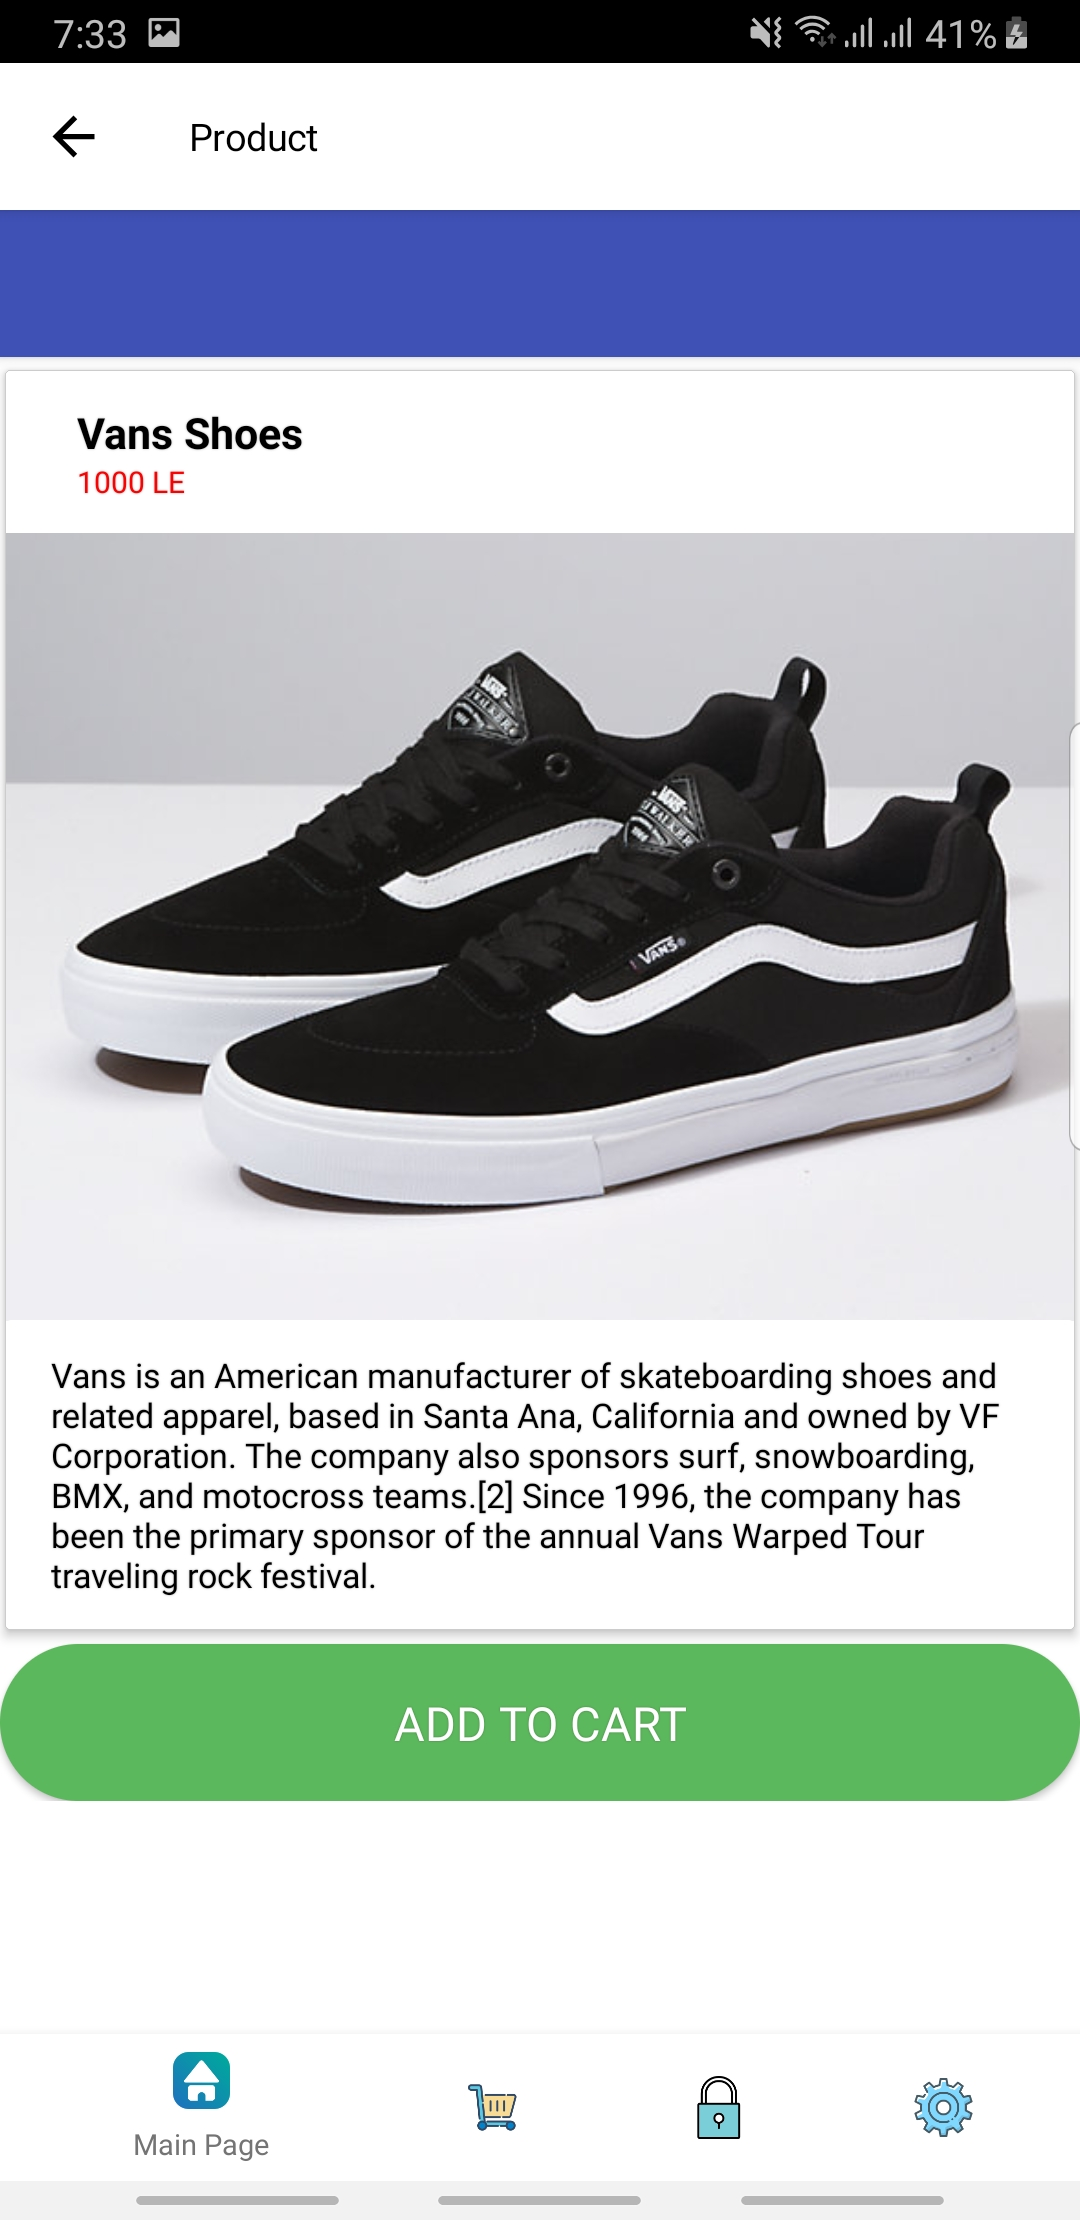
\includegraphics[width=0.5\textwidth]{images/Software/product.jpg}%
     % you need to add the caption for the list of figures
    \caption[Mobile Application: product Screen]{product Screen}\label{fig: productPageScreen}%
  \end{figure}\newpage
  
In Figure \ref{fig: Mobile Application:Cart Screen} each user has its own cart with different elements to buy the “proceed to check out” button redirects the user to Stripe component.  
\newline
\begin{figure}[htp]%
    \center%
    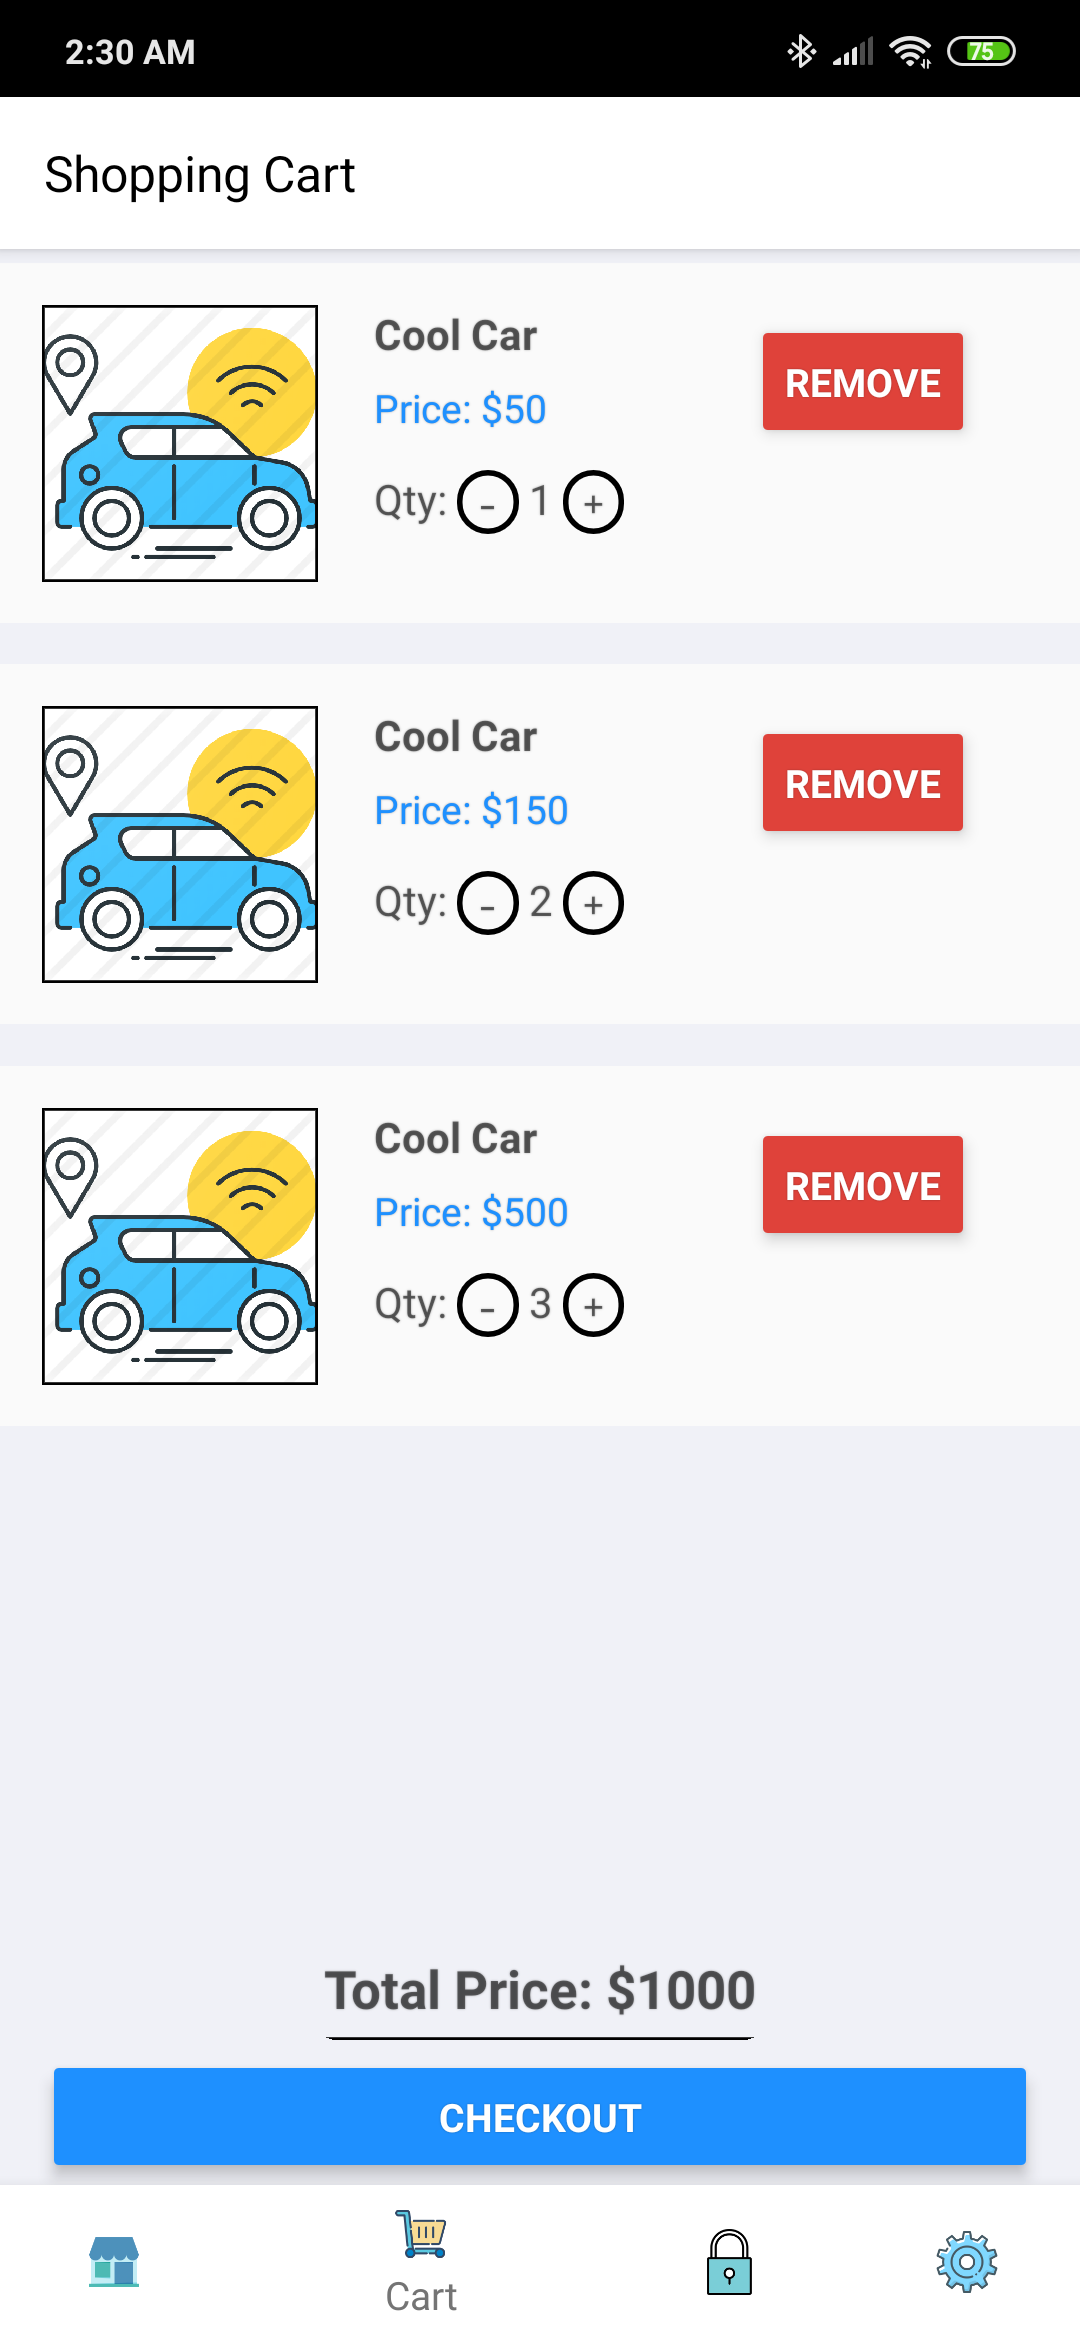
\includegraphics[width=0.44\textwidth]{images/Software/cartmobile.png}%
     % you need to add the caption for the list of figures
    \caption[Mobile Application:Cart Screen]{Mobile Application:Cart Screen}\label{fig: Mobile Application:Cart Screen}%
  \end{figure}
  
  
  

